
%% bare_jrnl.tex
%% V1.4b
%% 2015/08/26
%% by Michael Shell
%% see http://www.michaelshell.org/
%% for current contact information.
%%
%% This is a skeleton file demonstrating the use of IEEEtran.cls
%% (requires IEEEtran.cls version 1.8b or later) with an IEEE
%% journal paper.
%%
%% Support sites:
%% http://www.michaelshell.org/tex/ieeetran/
%% http://www.ctan.org/pkg/ieeetran
%% and
%% http://www.ieee.org/

%%*************************************************************************
%% Legal Notice:
%% This code is offered as-is without any warranty either expressed or
%% implied; without even the implied warranty of MERCHANTABILITY or
%% FITNESS FOR A PARTICULAR PURPOSE! 
%% User assumes all risk.
%% In no event shall the IEEE or any contributor to this code be liable for
%% any damages or losses, including, but not limited to, incidental,
%% consequential, or any other damages, resulting from the use or misuse
%% of any information contained here.
%%
%% All comments are the opinions of their respective authors and are not
%% necessarily endorsed by the IEEE.
%%
%% This work is distributed under the LaTeX Project Public License (LPPL)
%% ( http://www.latex-project.org/ ) version 1.3, and may be freely used,
%% distributed and modified. A copy of the LPPL, version 1.3, is included
%% in the base LaTeX documentation of all distributions of LaTeX released
%% 2003/12/01 or later.
%% Retain all contribution notices and credits.
%% ** Modified files should be clearly indicated as such, including  **
%% ** renaming them and changing author support contact information. **
%%*************************************************************************


% *** Authors should verify (and, if needed, correct) their LaTeX system  ***
% *** with the testflow diagnostic prior to trusting their LaTeX platform ***
% *** with production work. The IEEE's font choices and paper sizes can   ***
% *** trigger bugs that do not appear when using other class files.       ***                          ***
% The testflow support page is at:
% http://www.michaelshell.org/tex/testflow/



\documentclass[journal]{IEEEtran}
%
% If IEEEtran.cls has not been installed into the LaTeX system files,
% manually specify the path to it like:
% \documentclass[journal]{../sty/IEEEtran}





% Some very useful LaTeX packages include:
% (uncomment the ones you want to load)


% *** MISC UTILITY PACKAGES ***
%
%\usepackage{ifpdf}
% Heiko Oberdiek's ifpdf.sty is very useful if you need conditional
% compilation based on whether the output is pdf or dvi.
% usage:
% \ifpdf
%   % pdf code
% \else
%   % dvi code
% \fi
% The latest version of ifpdf.sty can be obtained from:
% http://www.ctan.org/pkg/ifpdf
% Also, note that IEEEtran.cls V1.7 and later provides a builtin
% \ifCLASSINFOpdf conditional that works the same way.
% When switching from latex to pdflatex and vice-versa, the compiler may
% have to be run twice to clear warning/error messages.


\usepackage{graphicx}
\usepackage{url}
\usepackage{mathtools}



% *** CITATION PACKAGES ***
%
%\usepackage{cite}
% cite.sty was written by Donald Arseneau
% V1.6 and later of IEEEtran pre-defines the format of the cite.sty package
% \cite{} output to follow that of the IEEE. Loading the cite package will
% result in citation numbers being automatically sorted and properly
% "compressed/ranged". e.g., [1], [9], [2], [7], [5], [6] without using
% cite.sty will become [1], [2], [5]--[7], [9] using cite.sty. cite.sty's
% \cite will automatically add leading space, if needed. Use cite.sty's
% noadjust option (cite.sty V3.8 and later) if you want to turn this off
% such as if a citation ever needs to be enclosed in parenthesis.
% cite.sty is already installed on most LaTeX systems. Be sure and use
% version 5.0 (2009-03-20) and later if using hyperref.sty.
% The latest version can be obtained at:
% http://www.ctan.org/pkg/cite
% The documentation is contained in the cite.sty file itself.






% *** GRAPHICS RELATED PACKAGES ***
%
\ifCLASSINFOpdf
  % \usepackage[pdftex]{graphicx}
  % declare the path(s) where your graphic files are
  % \graphicspath{{../pdf/}{../jpeg/}}
  % and their extensions so you won't have to specify these with
  % every instance of \includegraphics
  % \DeclareGraphicsExtensions{.pdf,.jpeg,.png}
\else
  % or other class option (dvipsone, dvipdf, if not using dvips). graphicx
  % will default to the driver specified in the system graphics.cfg if no
  % driver is specified.
  % \usepackage[dvips]{graphicx}
  % declare the path(s) where your graphic files are
  % \graphicspath{{../eps/}}
  % and their extensions so you won't have to specify these with
  % every instance of \includegraphics
  % \DeclareGraphicsExtensions{.eps}
\fi
% graphicx was written by David Carlisle and Sebastian Rahtz. It is
% required if you want graphics, photos, etc. graphicx.sty is already
% installed on most LaTeX systems. The latest version and documentation
% can be obtained at: 
% http://www.ctan.org/pkg/graphicx
% Another good source of documentation is "Using Imported Graphics in
% LaTeX2e" by Keith Reckdahl which can be found at:
% http://www.ctan.org/pkg/epslatex
%
% latex, and pdflatex in dvi mode, support graphics in encapsulated
% postscript (.eps) format. pdflatex in pdf mode supports graphics
% in .pdf, .jpeg, .png and .mps (metapost) formats. Users should ensure
% that all non-photo figures use a vector format (.eps, .pdf, .mps) and
% not a bitmapped formats (.jpeg, .png). The IEEE frowns on bitmapped formats
% which can result in "jaggedy"/blurry rendering of lines and letters as
% well as large increases in file sizes.
%
% You can find documentation about the pdfTeX application at:
% http://www.tug.org/applications/pdftex





% *** MATH PACKAGES ***
%
%\usepackage{amsmath}
% A popular package from the American Mathematical Society that provides
% many useful and powerful commands for dealing with mathematics.
%
% Note that the amsmath package sets \interdisplaylinepenalty to 10000
% thus preventing page breaks from occurring within multiline equations. Use:
%\interdisplaylinepenalty=2500
% after loading amsmath to restore such page breaks as IEEEtran.cls normally
% does. amsmath.sty is already installed on most LaTeX systems. The latest
% version and documentation can be obtained at:
% http://www.ctan.org/pkg/amsmath





% *** SPECIALIZED LIST PACKAGES ***
%
%\usepackage{algorithmic}
% algorithmic.sty was written by Peter Williams and Rogerio Brito.
% This package provides an algorithmic environment fo describing algorithms.
% You can use the algorithmic environment in-text or within a figure
% environment to provide for a floating algorithm. Do NOT use the algorithm
% floating environment provided by algorithm.sty (by the same authors) or
% algorithm2e.sty (by Christophe Fiorio) as the IEEE does not use dedicated
% algorithm float types and packages that provide these will not provide
% correct IEEE style captions. The latest version and documentation of
% algorithmic.sty can be obtained at:
% http://www.ctan.org/pkg/algorithms
% Also of interest may be the (relatively newer and more customizable)
% algorithmicx.sty package by Szasz Janos:
% http://www.ctan.org/pkg/algorithmicx




% *** ALIGNMENT PACKAGES ***
%
%\usepackage{array}
% Frank Mittelbach's and David Carlisle's array.sty patches and improves
% the standard LaTeX2e array and tabular environments to provide better
% appearance and additional user controls. As the default LaTeX2e table
% generation code is lacking to the point of almost being broken with
% respect to the quality of the end results, all users are strongly
% advised to use an enhanced (at the very least that provided by array.sty)
% set of table tools. array.sty is already installed on most systems. The
% latest version and documentation can be obtained at:
% http://www.ctan.org/pkg/array


% IEEEtran contains the IEEEeqnarray family of commands that can be used to
% generate multiline equations as well as matrices, tables, etc., of high
% quality.




% *** SUBFIGURE PACKAGES ***
%\ifCLASSOPTIONcompsoc
%  \usepackage[caption=false,font=normalsize,labelfont=sf,textfont=sf]{subfig}
%\else
%  \usepackage[caption=false,font=footnotesize]{subfig}
%\fi
% subfig.sty, written by Steven Douglas Cochran, is the modern replacement
% for subfigure.sty, the latter of which is no longer maintained and is
% incompatible with some LaTeX packages including fixltx2e. However,
% subfig.sty requires and automatically loads Axel Sommerfeldt's caption.sty
% which will override IEEEtran.cls' handling of captions and this will result
% in non-IEEE style figure/table captions. To prevent this problem, be sure
% and invoke subfig.sty's "caption=false" package option (available since
% subfig.sty version 1.3, 2005/06/28) as this is will preserve IEEEtran.cls
% handling of captions.
% Note that the Computer Society format requires a larger sans serif font
% than the serif footnote size font used in traditional IEEE formatting
% and thus the need to invoke different subfig.sty package options depending
% on whether compsoc mode has been enabled.
%
% The latest version and documentation of subfig.sty can be obtained at:
% http://www.ctan.org/pkg/subfig




% *** FLOAT PACKAGES ***
%
%\usepackage{fixltx2e}
% fixltx2e, the successor to the earlier fix2col.sty, was written by
% Frank Mittelbach and David Carlisle. This package corrects a few problems
% in the LaTeX2e kernel, the most notable of which is that in current
% LaTeX2e releases, the ordering of single and double column floats is not
% guaranteed to be preserved. Thus, an unpatched LaTeX2e can allow a
% single column figure to be placed prior to an earlier double column
% figure.
% Be aware that LaTeX2e kernels dated 2015 and later have fixltx2e.sty's
% corrections already built into the system in which case a warning will
% be issued if an attempt is made to load fixltx2e.sty as it is no longer
% needed.
% The latest version and documentation can be found at:
% http://www.ctan.org/pkg/fixltx2e


%\usepackage{stfloats}
% stfloats.sty was written by Sigitas Tolusis. This package gives LaTeX2e
% the ability to do double column floats at the bottom of the page as well
% as the top. (e.g., "\begin{figure*}[!b]" is not normally possible in
% LaTeX2e). It also provides a command:
%\fnbelowfloat
% to enable the placement of footnotes below bottom floats (the standard
% LaTeX2e kernel puts them above bottom floats). This is an invasive package
% which rewrites many portions of the LaTeX2e float routines. It may not work
% with other packages that modify the LaTeX2e float routines. The latest
% version and documentation can be obtained at:
% http://www.ctan.org/pkg/stfloats
% Do not use the stfloats baselinefloat ability as the IEEE does not allow
% \baselineskip to stretch. Authors submitting work to the IEEE should note
% that the IEEE rarely uses double column equations and that authors should try
% to avoid such use. Do not be tempted to use the cuted.sty or midfloat.sty
% packages (also by Sigitas Tolusis) as the IEEE does not format its papers in
% such ways.
% Do not attempt to use stfloats with fixltx2e as they are incompatible.
% Instead, use Morten Hogholm'a dblfloatfix which combines the features
% of both fixltx2e and stfloats:
%
% \usepackage{dblfloatfix}
% The latest version can be found at:
% http://www.ctan.org/pkg/dblfloatfix




%\ifCLASSOPTIONcaptionsoff
%  \usepackage[nomarkers]{endfloat}
% \let\MYoriglatexcaption\caption
% \renewcommand{\caption}[2][\relax]{\MYoriglatexcaption[#2]{#2}}
%\fi
% endfloat.sty was written by James Darrell McCauley, Jeff Goldberg and 
% Axel Sommerfeldt. This package may be useful when used in conjunction with 
% IEEEtran.cls'  captionsoff option. Some IEEE journals/societies require that
% submissions have lists of figures/tables at the end of the paper and that
% figures/tables without any captions are placed on a page by themselves at
% the end of the document. If needed, the draftcls IEEEtran class option or
% \CLASSINPUTbaselinestretch interface can be used to increase the line
% spacing as well. Be sure and use the nomarkers option of endfloat to
% prevent endfloat from "marking" where the figures would have been placed
% in the text. The two hack lines of code above are a slight modification of
% that suggested by in the endfloat docs (section 8.4.1) to ensure that
% the full captions always appear in the list of figures/tables - even if
% the user used the short optional argument of \caption[]{}.
% IEEE papers do not typically make use of \caption[]'s optional argument,
% so this should not be an issue. A similar trick can be used to disable
% captions of packages such as subfig.sty that lack options to turn off
% the subcaptions:
% For subfig.sty:
% \let\MYorigsubfloat\subfloat
% \renewcommand{\subfloat}[2][\relax]{\MYorigsubfloat[]{#2}}
% However, the above trick will not work if both optional arguments of
% the \subfloat command are used. Furthermore, there needs to be a
% description of each subfigure *somewhere* and endfloat does not add
% subfigure captions to its list of figures. Thus, the best approach is to
% avoid the use of subfigure captions (many IEEE journals avoid them anyway)
% and instead reference/explain all the subfigures within the main caption.
% The latest version of endfloat.sty and its documentation can obtained at:
% http://www.ctan.org/pkg/endfloat
%
% The IEEEtran \ifCLASSOPTIONcaptionsoff conditional can also be used
% later in the document, say, to conditionally put the References on a 
% page by themselves.




% *** PDF, URL AND HYPERLINK PACKAGES ***
%
%\usepackage{url}
% url.sty was written by Donald Arseneau. It provides better support for
% handling and breaking URLs. url.sty is already installed on most LaTeX
% systems. The latest version and documentation can be obtained at:
% http://www.ctan.org/pkg/url
% Basically, \url{my_url_here}.




% *** Do not adjust lengths that control margins, column widths, etc. ***
% *** Do not use packages that alter fonts (such as pslatex).         ***
% There should be no need to do such things with IEEEtran.cls V1.6 and later.
% (Unless specifically asked to do so by the journal or conference you plan
% to submit to, of course. )


% correct bad hyphenation here
\hyphenation{op-tical net-works semi-conduc-tor}


\begin{document}
%
% paper title
% Titles are generally capitalized except for words such as a, an, and, as,
% at, but, by, for, in, nor, of, on, or, the, to and up, which are usually
% not capitalized unless they are the first or last word of the title.
% Linebreaks \\ can be used within to get better formatting as desired.
% Do not put math or special symbols in the title.
\title{Clinical Pneumonia Classification via Multimodal Data Fusion}
%
%
% author names and IEEE memberships
% note positions of commas and nonbreaking spaces ( ~ ) LaTeX will not break
% a structure at a ~ so this keeps an author's name from being broken across
% two lines.
% use \thanks{} to gain access to the first footnote area
% a separate \thanks must be used for each paragraph as LaTeX2e's \thanks
% was not built to handle multiple paragraphs
%

\author{Michael~Shell,~\IEEEmembership{Member,~IEEE,}
        John~Doe,~\IEEEmembership{Fellow,~OSA,}
        and~Jane~Doe,~\IEEEmembership{Life~Fellow,~IEEE}% <-this % stops a space
\thanks{M. Shell was with the Department
of Electrical and Computer Engineering, Georgia Institute of Technology, Atlanta,
GA, 30332 USA e-mail: (see http://www.michaelshell.org/contact.html).}% <-this % stops a space
\thanks{J. Doe and J. Doe are with Anonymous University.}% <-this % stops a space
\thanks{Manuscript received April 19, 2005; revised August 26, 2015.}}

% note the % following the last \IEEEmembership and also \thanks - 
% these prevent an unwanted space from occurring between the last author name
% and the end of the author line. i.e., if you had this:
% 
% \author{....lastname \thanks{...} \thanks{...} }
%                     ^------------^------------^----Do not want these spaces!
%
% a space would be appended to the last name and could cause every name on that
% line to be shifted left slightly. This is one of those "LaTeX things". For
% instance, "\textbf{A} \textbf{B}" will typeset as "A B" not "AB". To get
% "AB" then you have to do: "\textbf{A}\textbf{B}"
% \thanks is no different in this regard, so shield the last } of each \thanks
% that ends a line with a % and do not let a space in before the next \thanks.
% Spaces after \IEEEmembership other than the last one are OK (and needed) as
% you are supposed to have spaces between the names. For what it is worth,
% this is a minor point as most people would not even notice if the said evil
% space somehow managed to creep in.



% The paper headers
\markboth{Journal of \LaTeX\ Class Files,~Vol.~14, No.~8, August~2015}%
{Shell \MakeLowercase{\textit{et al.}}: Bare Demo of IEEEtran.cls for IEEE Journals}
% The only time the second header will appear is for the odd numbered pages
% after the title page when using the twoside option.
% 
% *** Note that you probably will NOT want to include the author's ***
% *** name in the headers of peer review papers.                   ***
% You can use \ifCLASSOPTIONpeerreview for conditional compilation here if
% you desire.




% If you want to put a publisher's ID mark on the page you can do it like
% this:
%\IEEEpubid{0000--0000/00\$00.00~\copyright~2015 IEEE}
% Remember, if you use this you must call \IEEEpubidadjcol in the second
% column for its text to clear the IEEEpubid mark.



% use for special paper notices
%\IEEEspecialpapernotice{(Invited Paper)}




% make the title area
\maketitle

% As a general rule, do not put math, special symbols or citations
% in the abstract or keywords.
\begin{abstract}

  Objective: Existing CAD(Computer Aided Detection) systems for pneumonia diagnosis are basically designed for chest X-ray image. But in clinical practice, CT(Computed Tomography) can provide more information and details which can help to increase the accuracy of diagnosing. Applying deep learning methods directly to raw CT scans requires much resources of computing. Moreover, patients' clinical information are often ignored in recent deep learning methods, which is conflicted to clinical practice. The objective of this paper is to effectively address the problems of absent of clinical information in deep learning methods and therefore to accurately diagnosis pneumonia via raw CT scans.
  Method: We imitate the radiologists' clinical diagnosis process and propose a novel model, MMDD(Multimodal Data Diagnosis), which combines CT visual features with patients' age, gender and complaints. 
  In MMDD, we treat process of reading CT scans as playing short videos and use RCNN(Recurrent Convolutional Neural Network) to capture visual features from CT image data. Meanwhile, complaints will be transformed into word vectors using word2vec and analyzed by LSTM(Long Short Term Memory). Visual features and complaint textual features will be fused together with patients' information about age and gender. All information above will play its role in the decision making process.
  In order to provide more visual features to MMDD, we extract images from three different ranges of HU values based on original CT scans and transform 1-channel grey level CT images into three-channel false color RGB images. Moreover, we use a auxiliary loss to enhance the gradient propagated to CNN. 
  Our model achieves 0.945 in accuracy, and has a very balanced performance in sensitivity and specificity. As far as we know, we are the first to classify pneumonic cases based on large scale clinical raw data using multimodal clinical data.
\end{abstract}

% Note that keywords are not normally used for peerreview papers.
\begin{IEEEkeywords}
Long Short Term Memory(LSTM), Pneumonia Diagnosis, Recurrent Convolutional Neural Network, Computed tomography (CT), Computer-aided detection and diagnosis (CAD), Multimodal Data
\end{IEEEkeywords}






% For peer review papers, you can put extra information on the cover
% page as needed:
% \ifCLASSOPTIONpeerreview
% \begin{center} \bfseries EDICS Category: 3-BBND \end{center}
% \fi
%
% For peerreview papers, this IEEEtran command inserts a page break and
% creates the second title. It will be ignored for other modes.
\IEEEpeerreviewmaketitle



\section{Introduction}
% The very first letter is a 2 line initial drop letter followed
% by the rest of the first word in caps.
% 
% form to use if the first word consists of a single letter:
% \IEEEPARstart{A}{demo} file is ....
% 
% form to use if you need the single drop letter followed by
% normal text (unknown if ever used by the IEEE):
% \IEEEPARstart{A}{}demo file is ....
% 
% Some journals put the first two words in caps:
% \IEEEPARstart{T}{his demo} file is ....
% 
% Here we have the typical use of a "T" for an initial drop letter
% and "HIS" in caps to complete the first word.
\IEEEPARstart{C}{hest} X-rays used to be the best available method for diagnosing pneumonia, played a crucial role in clinical care\cite{Franquet2001Imaging} and epidemiological studies\cite{Thomas2005Standardized}. However, with the development of economic and technology, CT(Computed Tomography) has become a common technology for diagnosing pneumonia. Compared to chest X-ray, CT can provide more detailed information which can help to diagnosis pneumonia in early stage and avoid delayed treatment.

According to the survey, a radiologist of a major hospital need to read hundreds scans of CT every day. Thus, developing a fast, robust and accurate CAD system to perform automated diagnosis of pneumonia is meaningful and important. 

There have been lots of models designed for diagnosing thoracic diseases.
Hoo-Chang Shin \cite{Shin2016Learning} combined CNN and LSTM\cite{hochreiter1997long}, proposed a model which could describe the contexts of a detected diseases based on the deep CNN features. This model used CNN to extract features from chest X-Ray and used LSTM to generated MeSH\cite{timmurphy.org} terms for chest X-Ray. In 2017, Xiaosong Wang et al.\cite{Wang2017ChestX} provided hospital-scale chest X-ray database ChestX-ray8 which contained eight common thoracic diseases. This database allowed researchers use deeper neural network to analyze thoracic diseases. They used different pre-trained CNN models on this dataset. Experiments showed that ResNet50 achieved highest AUROC score 0.6333. They also provided ChestX-ray14 with more kinds of thoracic diseases.
Based on this database, later in 2017, Yao et al.\cite{yao2017learning} achieved 0.713 in AUROC score using DenseNet Image Encoder. Pranav Rajpurkar, Andrew Y. Ng et al. \cite{Rajpurkar2017CheXNet} developed CheXnet with 121 convolutional layers and achieved 0.7680 in AUROC.
In 2018, Xiaosong Wang et al.\cite{Wang2018TieNet} proposed TieNet, which could classify the chest X-Rays into different diseases and generate the report at the same time. In TieNet, CNN was used capture features of chest X-Rays, RNN learned these features and generated report based on attention mechanism, which could help model to focus on different parts of chest X-Ray alone with the generation of reports. 

Studies above have something in common. First of all, they were designed for chest X-Rays, which means even if they can achieve good results in every indication, these models still cannot handle CT(Computed Tomography) scans, which can provide more detailed visual information. CT scans have a clearer view of patients' bodies, since bones, skin, vessels, mediastinal and lung tissues may cause overlapping shadows in chest X-ray and cause misdiagnosis.
Each slice in CT scans is a 2-D image of human body scan, using these 2-D slices can reconstruct 3-D structure of human bodies. 
Extensive studies show that 3-D CNN is the best choice for keeping 3-D spatial information in CT\cite{Yorozu1987Electron}. However, 3-D CNN cannot be applied to raw CT data directly since it will bring a heavy burden to the server. Radiologists need to accurately measure the lesions, so we cannot reduce the size of images by resizing at will.
 
Second, these models are not designed following the radiologists' diagnosing process but are designed for the convenience of computer vision studies and deep learning model training. For models like CheXnet, image information is the key of models. Few of them combine image visual features with clinical information. Models like TieNet do combine image visual features with descriptions about images written by radiologists. But these descriptions only provide information related to images, which means no extra clinical information is provided to models. We also believe using descriptions about images written by radiologists to improve models is not quite convincing, since descriptions like `Findings' and `impressions' sometimes include diagnosis conclusions.
Patients' complaints is a very useful information when doctors are diagnosing, since complaints is patients' direct feeling about their physical condition. Moreover, information of age and gender is also related to some certain diseases. However, as far as we know, few studies use this information to improve the performance of CAD systems. 

In general, there are two major problems of existing CAD systems: (1) They cannot handle raw CT scans, and this problem has become a practical limitation of deep learning models designed for medical problems; (2) Few studies consider clinical information like patients' complaints, which is conflict to clinical practice.

In this study, we use raw data collected from The First Affiliated Hospital of Army Medical University, each case contains not only CT image information, but also clinical information about patient gender, age and complaints. 
We treat slices of CT scans as video frames, and transform the problems of analyzing CT scans into the problems of analyzing short videos. We use RCNN(Recurrent Convolutional Neural Network) to extract features from slices of CT scans. Then we embed patients' complaints into word vectors using word2vec\cite{mikolov2013efficient}\cite{mikolov2013distributed}. We use another LSTM(Long Short Term Memory) to extract textual features, and concatenate it with features of images, alone with information about patients' age and gender. Our mode Multimodal Data Diagnosis(MMDD) model, as shown in Fig~\ref{MMDD}, will learn a joint distribution of all features above and gives out the final classification result.

Our main contributions are listed as follow:

(1) We design a protocol for selecting particular series of scans from raw CT data collected from Radiology Department of The First Affiliated Hospital of Army Medical University, according to `Slice Thickness' and `Convolution Kernels' and transform original CT images into HU value matrices for future use. 

(2) We transform CT images from one-channel grey level images into three-channel fake color images using three different ranges of HU values, and analyze the effectiveness of three-channel fake color images via middle outputs of CNN.

(3) We propose a novel model: MMDD(Multimodal Data Diagnosis). This model can capture visual features by playing CT slices as short videos. Meanwhile, MMDD will fuse visual features with clinical information like patient complaint, age and gender to predict whether these cases are pneumonic.

The remainder of the manuscript is organized as follows. 
Section~\ref{methodology} describes the architecture of MMDD and details of our model.
Section~\ref{experiments} describes the pre-processing steps of dataset and reports our experimental results.
Section~\ref{discuss} further discusses some key points of proposed model and some phenomenons shown during experiments.
Our conclusions are drawn in section~\ref{conclude}.

\section{Methodology}
\label{methodology}

\subsection{Construction of Recurrent Convolutional Neural Network}
\label{RCNN}
RCNN(Recurrent Convolutional Neural Network) has been proved to be very useful for video caption, description and classification \cite{Donahue2015Long}\cite{Aafaq2019Spatio}, however, only a few work apply RCNN to medical image analyze. Zreik, Majd et al. \cite{Zreik2018A} recently use RCNN for automatic detection and classification of coronary artery plaque, they use CNN extracts features out of $ 25\times25\times25$ voxels cubes, and  use an RNN to process the entire sequence using gated recurrent units (GRUs)\cite{chung2014empirical}. They proved that RCNN's potential for sequence information processing of medical images. Meanwhile, slices of CT scans can be seen as video frames, so in this study, we use RCNN to capture visual features from CT slices.

Follow the study\cite{Donahue2015Long}, we use LSTM as our RNN cells cause LSTM has been demonstrated to be capable of large-scale learning of sequence data. However, few studies have paid attention to different CNN models' performance on medical images, so we test three kinds of classic CNN models: VGG\cite{simonyan2015very}, ResNet\cite{he2016deep} and GoogLeNet with Inception-V3 \cite{szegedy2016rethinking}. 
We wanted to test deeper models like ResNet101, but it will cost more resource of calculation so we give up. Experiments will be discussed in section~\ref{experiments} and section~\ref{discuss}.

We use CNN without fully-connected layers as feature extractor. The input size of CNN is $512 \times 512$, so the outputs of CNN will be very large. We use global average pooling\cite{lin2014network}, as shown in Fig~\ref{gap}, to greatly reduce the number of neurons. It is a replacement of fully-connected layers to enable the summing of spatial information of feature maps. After global average pooling, we insert a fully-connected layer to reduce dimensions to $256$ and fit the requirements of LSTM. Following study in \cite{Donahue2015Long}, the number of LSTM units is set to $256$.
\begin{figure}[htb]
    \centerline{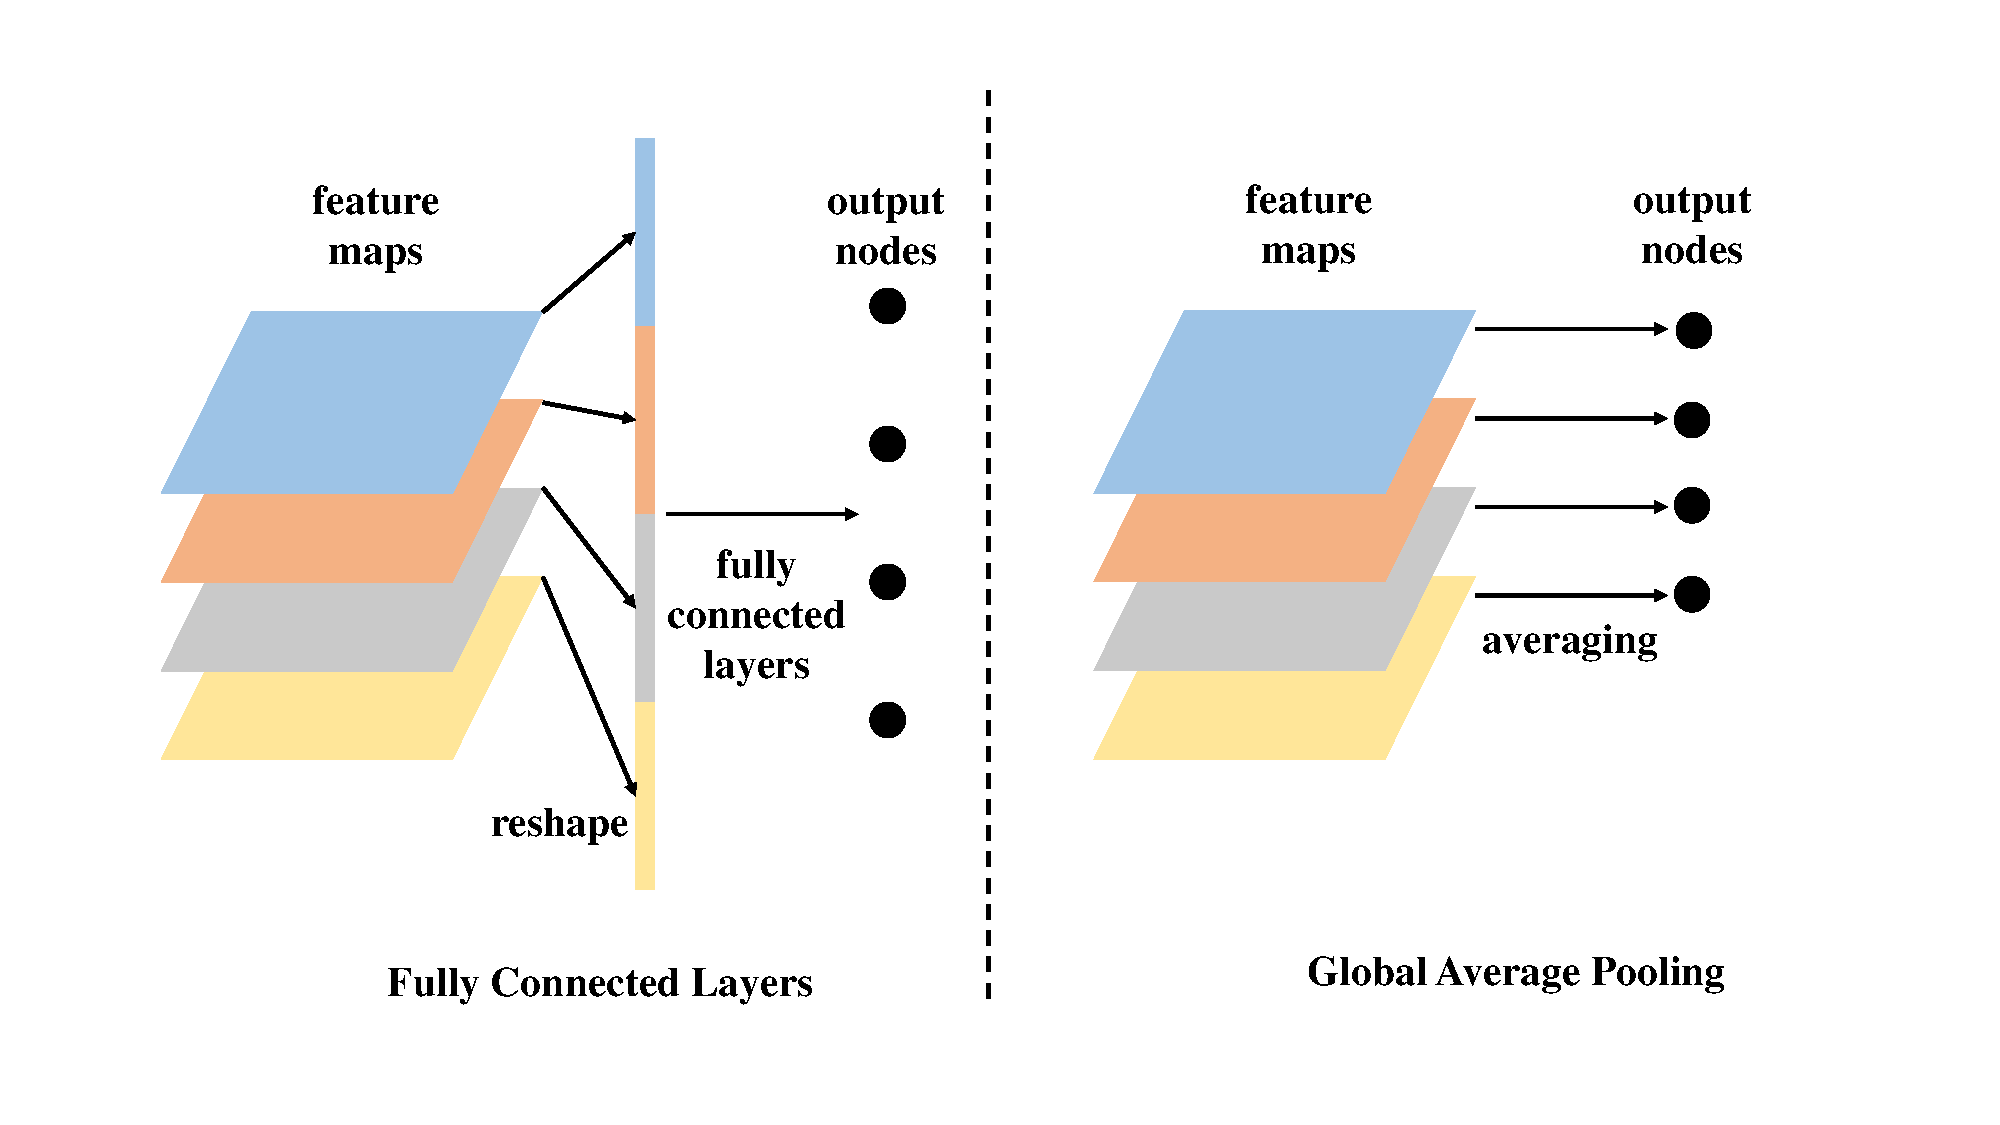
\includegraphics[width=100mm]{gap.pdf}}
    \vspace{-0cm}
    \caption{Difference between Fully Connected Layers and Global Average Pooling}
    \vspace{-0cm}
    \label{gap}
    \end{figure}

For example, if we use ResNet50, the final feature maps will be $16 \times 16 \times 2048$. If we use fully-connected layer, the length of first fully-connected layer will be $1 \times 524288$, which will make model very difficult to train. 
If we use global average pooling, outputs from CNN will be reshaped into a tensor of size $1 \times 2048$, then it will be easy to reduce the tensor to $1 \times 256$ using one fully-connected layer. If we have $n$ slice, we will have a matrix with size $n \times 256$, this matrix will be fed into LSTM by $n$ steps.

In order to get the best RCNN for CT scans, we run experiments to get the best combination between CNN models and LSTM. The experiments show that ResNet50 performs the best in these three models, so our RCNN use ResNet50 as its CNN part, and use one layer of LSTM cells as its RNN part. This conclusion is similar to \cite{Wang2017ChestX}, their experiments showed that ResNet50 outperformed GoogLeNet and VGG16.

In fact, LSTM layer plays the role of encoder, it encodes image feature sequences and gives out the output of the last step as middle state $hv_t$:
\begin{equation}
hv_t = LSTM(Fx_t, hv_{t-1}, z_{t-1})
\label{hvt}
\end{equation}
$Fx_t$ is the $t$-th visual features in CT slices, $hv_{t-1}$ is LSTM hidden state of $t-1$ step, $z_{t-1}$ is LSTM output of $t-1$ step. $t$ is the length of slices, in this study, $t$ is equal to 32.


\subsection{Multimodal Data Fusion and Multimodal Data Diagnosis}
\label{MMDD}
Besides CT image information, we also know patients gender, age, and complaints. For gender and age, we use them as additional features and set a tensor with size $1 \times 2$ to hold values. For patients' complaints, we will use Jieba Chinese word segmentation tool $\footnote[1]{https://github.com/fxsjy/jieba}$ to segment Chinese sentences into word sequences. This process steps will be discussed later in section~\ref{experiments}. We set length of Chinese word sequence to 16. Then we transform sequences of words into sequences of vectors using word2vec, which is commonly used in nature language process, since it can capture the relations between words. The width of vectors is set to 50, so does the number of LSTM units. This LSTM is the second encoder to encode complaint. It is calculated in the same way as Eq.~\ref{hvt}:
\begin{equation}
    hc_{ct} = LSTM(Cx_{ct}, hc_{ct-1}, z_{ct-1})
    \label{hct}
\end{equation}
$Cx_{ct}$ is word embedding matrix of the $ct$-th word in complaint, $hc_{ct-1}$ is LSTM hidden state of $ct-1$ step. $ct$ is the length of complaint, which is 16. 

We use cross-entropy as classification loss function\cite{Zreik2018A}. After getting $hv_t$, $hc_{ct}$, we can calculate the prediction and loss $\Phi_1$ as follows:
\begin{align*}\label{classifyandloss1}
    \Phi_1 &= \sum_i{y_i log(\Delta_i)}, \\
    \Delta &= Softmax(F(hv_t \bigotimes hc_{ct} \bigotimes A \bigotimes G))
\end{align*}

where $y_i$ are vectors for the labels of patients, $\Delta$ is prediction after Softmax, $\bigotimes$ is the concatenation operation, $A$ is patient age, $G$ is patient gender. $F$ is a function to calculate joint distributions of $hv_t$, $hc_{ct}$, $A$ and $G$. In this study, we use two fully-connected layers to fit the function.

Since LSTM need to encode 32 visual features, we assume that the gradients propagate to CNN will be very small, so that CNN will not be trained properly. Invoked by study in \cite{szegedy2016rethinking}, we use a auxiliary loss to enhance signal of gradient for CNN.
The auxiliary loss $\Phi_2$ and loss of whole model $Loss$ is defined as follow: 
\begin{align*}
Loss &=  (1 - \omega) \times \Phi_1 +  \omega \times \Phi_2 \\
\Phi_2 &= \sum_i{y_i log(\Delta^c_i)}
\end{align*}
where $\omega$ is a parameter within the interval (0, 1). $\Phi_2$ is classification cross-entropy loss from CNN, $\Delta^c_i$ is Softmax prediction of CNN. $\omega$ can adjust the weight of two losses at different training phases.
We expect that at the beginning of training, CNN get stronger gradient and learn to capture features from CT images more quickly. After parameters of CNN get stable, $\Phi_1$ tends to get small and keep updating parameters of LSTM. We output weights of two losses during training MMDD, as shown in Table~\ref{weights}, weight for LSTM loss ($1 - \omega$) is 0.6238 at the beginning of training(602 steps), however, W1 will increase to 0.7234 when training process comes to 36120 steps, it meas weight for CNN is 0.3762 at 602 steps, and it will drop to 0.2766 at the end. Experiments also show that RCNN with auxiliary loss can have a better performance, which will be discussed latter in section~\ref{experiments}.

Finally, a Multimodal Data Diagnosis(MMDD) is built, RCNN for image data and LSTM for complaints will be trained jointly, the architecture of MMDD is shown in Fig~\ref{MMDD}. 

\begin{figure*}[t]
    \centerline{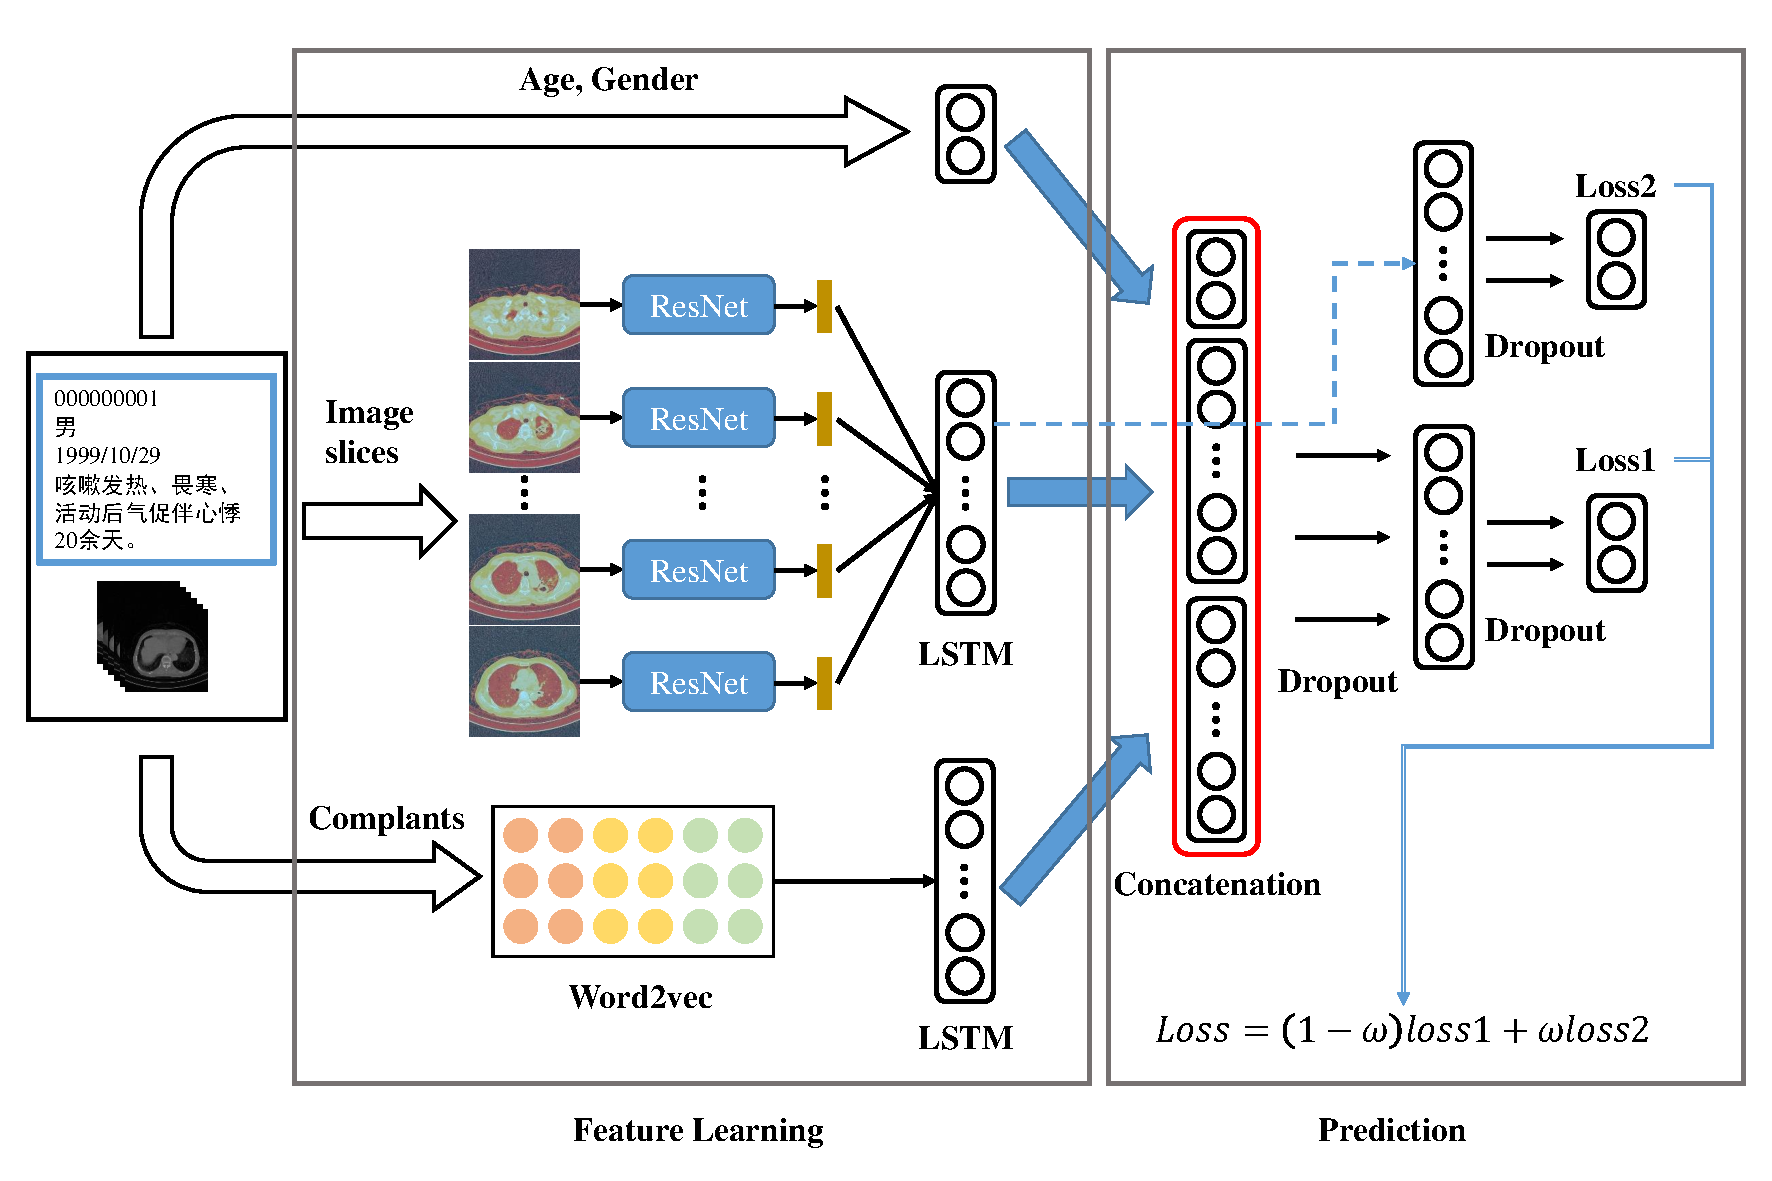
\includegraphics[width=160mm]{MMDD.pdf}}
    \vspace{-0cm}
    \caption{Multimodal Data Diagnosis Model}
    \vspace{-0cm}
    \label{MMDD}
    \end{figure*}

\begin{table}[t]
    \vspace{-0cm}
    \caption{Weights of Two Losses at Different Training Step}
    \vspace{-0cm}
    \begin{center}
    \begin{tabular}{|c|c|c|}
    \hline
    \textbf{\textit{Number of Steps}} & \textbf{\textit{$1 - \omega$}} & \textbf{\textit{$\omega$}}\\
    \hline
    602 &0.6238 & 0.3762  \\
    9030 &0.6547 & 0.3453  \\
    18060 &0.7027 & 0.2973  \\
    27090 &0.7185 & 0.2815  \\
    36120 &0.7234 & 0.2766  \\

    \hline
    \end{tabular}
    \vspace{-0cm}
    \label{weights}
    \end{center}
    \vspace{-0cm}
    \end{table}

\subsection{Training Process}
\label{trainingprocess}
There two steps during training process.
The first step is to train difference kinds of RCNN to get the best combination between CNN models and LSTM, the outputs from RCNN($1 \times 256$) will be feed into two fully connected layers to get classification results, as shown in Fig~\ref{onestream}. We compare three kinds of classic CNN models: VGG16, GoogLeNet with Inception-V3, ResNet50. VGG16 is relatively shallow, ResNet50 is deepest in these three kinds of models. We tried to use deeper network like ResNet101, however using ResNet101 make the training of model very slow and bring a heavy burden to servers. So we keep ResNet50 in RCNN.
\begin{figure*}[t]
    \centerline{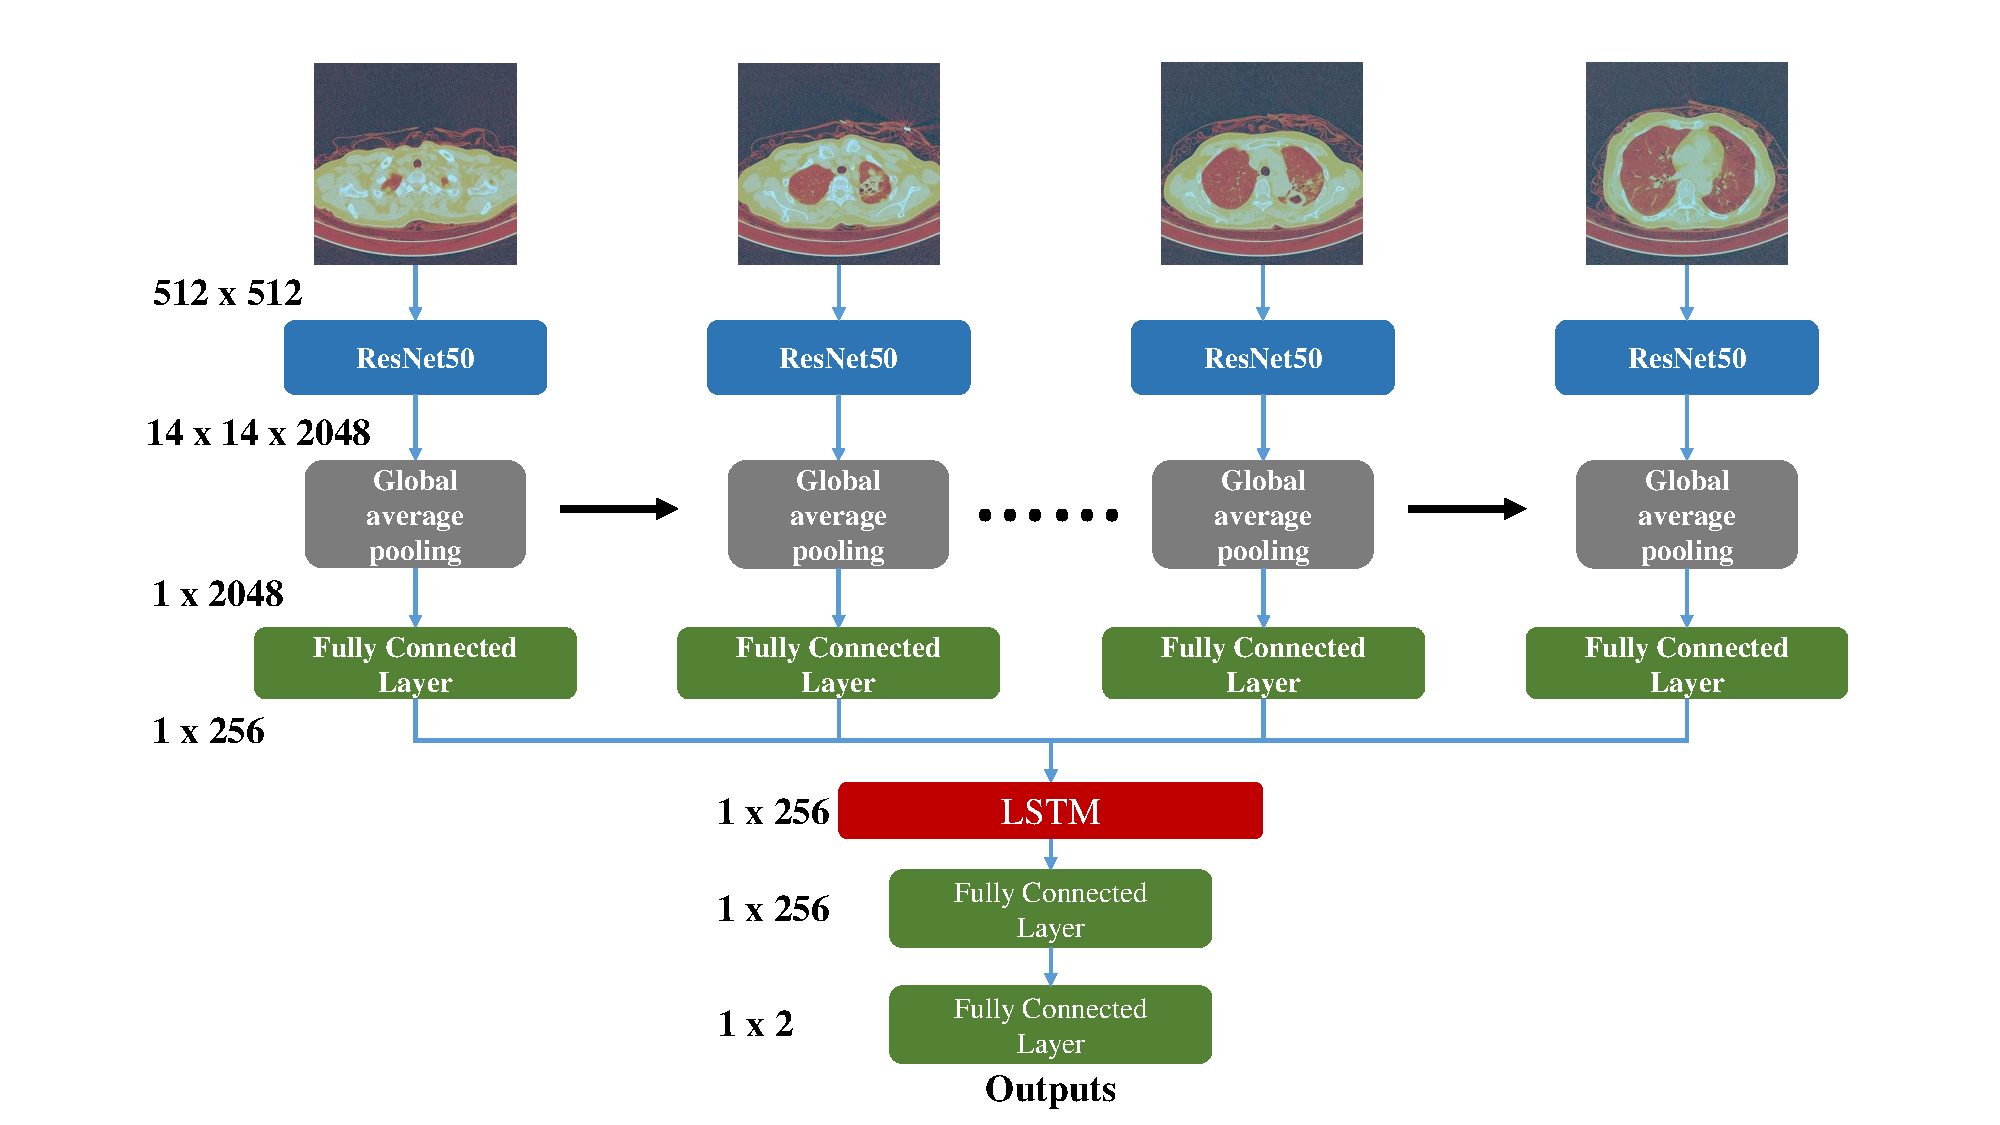
\includegraphics[width=150mm]{onestream.pdf}}
    \vspace{-0cm}
    \caption{Architecture of RCNN}
    \vspace{-0cm}
    \label{onestream}
    \end{figure*}

The second step is to train MMDD model. We use model get in the first step as encoder for CT scan visual features, use LSTM as feature encoder for complaints, and combine them with information of age and gender. All these features will be feed into two fully-connected layers and one Softmax layer to get final classification results. Initial learning rate is set 0.0005 and drops 50\% every 3000 training steps. The dropout rate in fully-connected layers is set to 0.5.

Moreover, we use CNN models pre-trained on ImageNet\cite{ILSVRC15}. Models without pre-training is almost impossible to train because it won't converge or converge very slow during training. We test difference RCNNs, and experiments show that using pre-trained models can significantly improve the converging speed, as shown in Fig~\ref{pretrain}.

Model will be trained for 4 epoch, and each epoch contains 15 iteration for all training data.

\begin{table}[htb]
    \vspace{-0cm}
    \caption{Comparison between Training from Scratch and Training with Pre-trained Weights}
    \vspace{-0cm}
    \begin{center}
        \begin{tabular}{|c|c|c|c|}
        \hline
        \textbf{\textit{Structure}} & \textbf{\textit{Pre-trained}} & \textbf{\textit{Data}}& \textbf{\textit{Accuracy}}  \\
        \hline
        RCNN(ResNet) &No & Lung Window Image & 0.545\\
        RCNN(GoogLeNet) & No & Lung Window Image & 0.545\\
        RCNN(ResNet) & Yes & Lung Window Image & 0.925\\
        RCNN(GoogLeNet) & Yes & Lung Window Image & 0.865\\
        
        \hline
        \end{tabular}
    \vspace{-0cm}
    \label{pretrain}
    \end{center}
    \vspace{-0cm}
    \end{table}


\section{Experiments}
\label{experiments}

\subsection{CT Image Data and Multimodal Data Generation}
\label{ctimagedata}
Because of the shortage of public CT dataset for pneumonia, we use raw data from Radiology Department of The First Affiliated Hospital of Army Medical University. We get 1036 cases of CT(842 cases with pneumonia, 464 healthy cases) from hospital PACS(Picture Archiving and Communication Systems). Open a CT scan with RadiAnt DICOM Viewer$\footnote[2]{www.radiantviewer.com}$, as shown in Fig~\ref{reader}, we can see that raw data from hospital may have more than one series of images(yellow rectangle), each series may have different data type or different image windows. Generally speaking, radiologists and doctors will use series with smallest `Slice Thickness', but for deep learning models, we need to pick up the most suitable series manually. This work is very heavy, so we design a protocol to let the computer pick up data for us.

\begin{figure}[t]
    \centerline{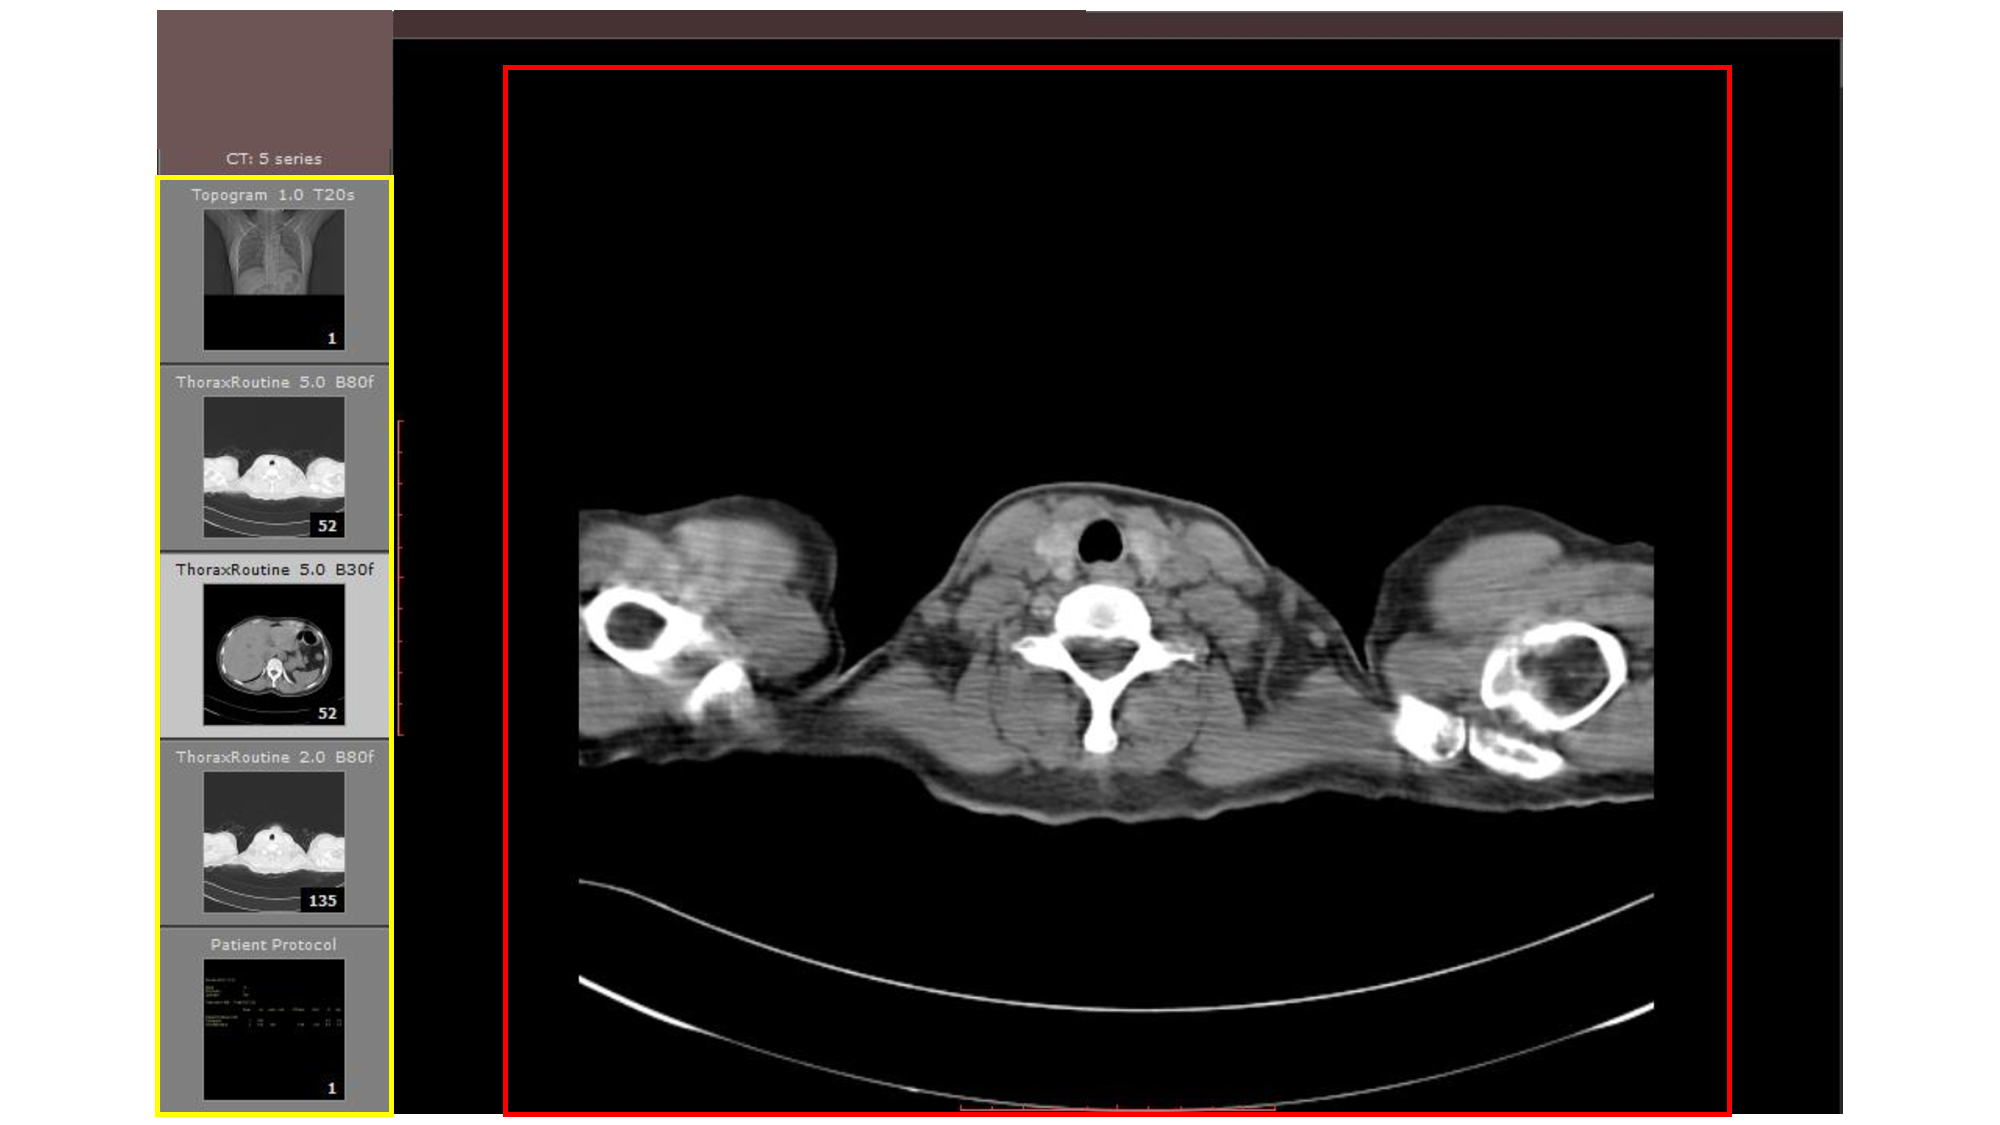
\includegraphics[width=90mm]{reader.pdf}}
    \vspace{-0cm}
    \caption{Structure of Raw Data from Hospital}
    \vspace{-0cm}
    \label{reader}
    \end{figure}


First of all, we eliminate these cases which start scanning from the middle of the chest. Then we pick up the best series from the whole cases according to the following requirements:

1. We use the series with the specific `Convolution Kernel'. Specific `Convolution Kernel' can make the CT more suitable for observing the lungs or chest, for example, in Fig~\ref{Bs}, slice under `B70s' has clearer view of lungs, slice under `B41s' has clearer view of heart. We need to notice that these names of `Convolution Kernel' vary between hospitals and CT equipments, so if you want to adopt this protocol, you need to observe `Convolution Kernel' in your environment. In our study, we choose `B31f', `I31f 3', `B70f', `B80f', `B70s', since radiologists use these `Convolution Kernel'  more frequently to observe the lungs and chest than other kinds of `Convolutional Kernel'. Number of different `Convolution Kernel' is shown in Fig~\ref{NumberofDifferentConvolutionKernel}. Other kinds of `Convolution Kernel' will be eliminated since series with other kinds of `Convolution Kernel' may have different perspectives of chest.
However, different `Convolution Kernel' will not affect images we analyze in the end, because all slices will be calculated and transformed into HU value matrices, which will be discussed in this Section.

\begin{figure}[t]
    \centerline{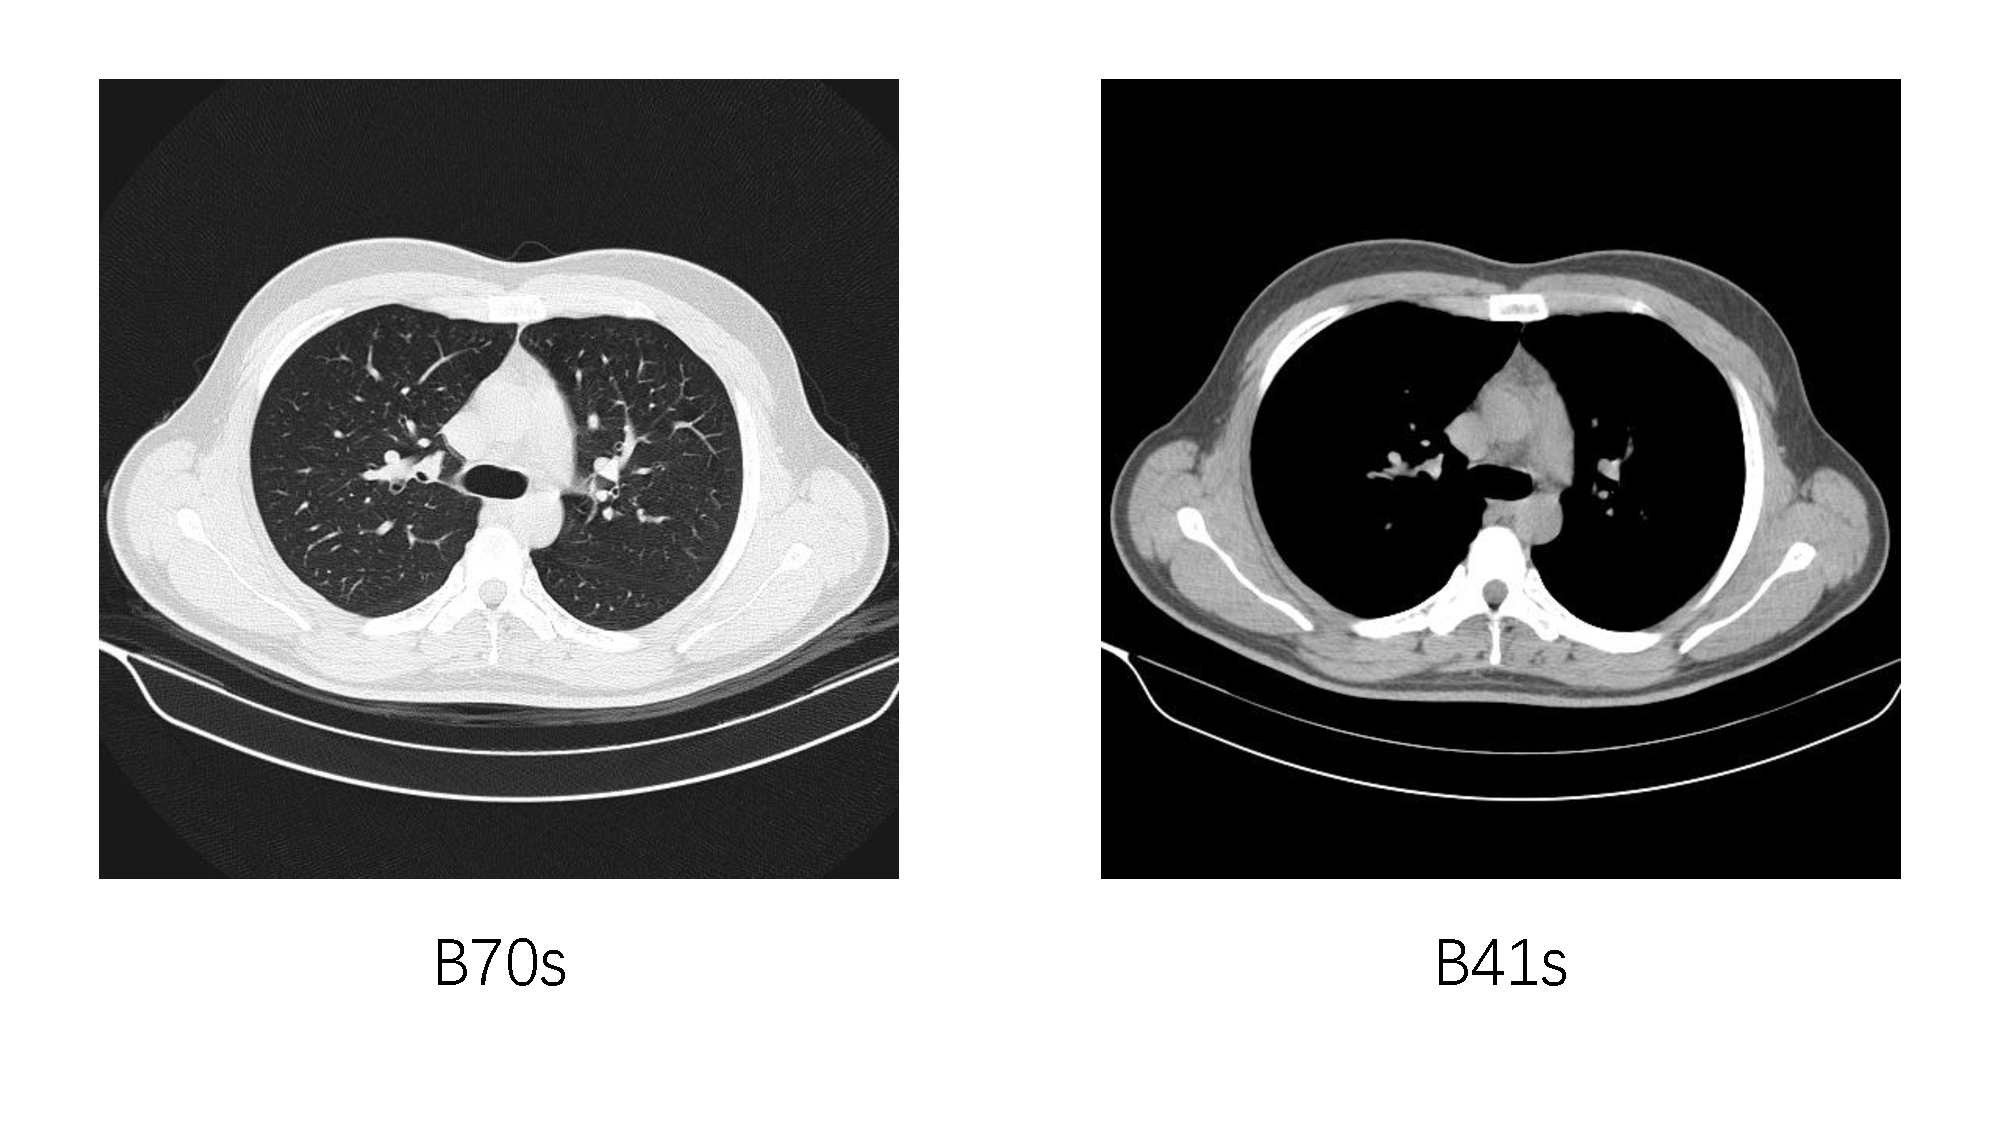
\includegraphics[width=100mm]{Bs.pdf}}
    \vspace{-0cm}
    \caption{Scans under Different Convolutional Kernel}
    \vspace{-0cm}
    \label{Bs}
    \end{figure}

2. We calculate `Slice Thickness' of each series, and keep series with the smallest `Slice Thickness', since small thickness may keep more detailed information of body structure. 

3. If there were more than one series meet the last two requirements, we will keep the series with the largest number of slices, which can have a larger span of view.

As a result, we keep 552 cases with pneumonia and 450 cases of healthy people (1002 cases total).
We split dataset in training/validation/testing as 60\% /20\% /20\% and make them identically distributed in three parts of datasets, so we have 602 cases in training set, 200 cases in validation set, 200 cases in test set.
Number of healthy and pneumonic cases in different slice-thickness is shown in Table~\ref{distributionofhealthyandpneumonic}.

Each CT scan has a case file. In case files, we can get patient basic information: patient ID, gender, age and complaint. Patient complaints are descriptions from patients which describe their own feeling about their condition, which is very important in clinical practice. In this study, we will use gender, age as additional features, and use LSTM extract textual features from patients' complaints, and combine them with features from CT slices.

\begin{figure}[t]
\centerline{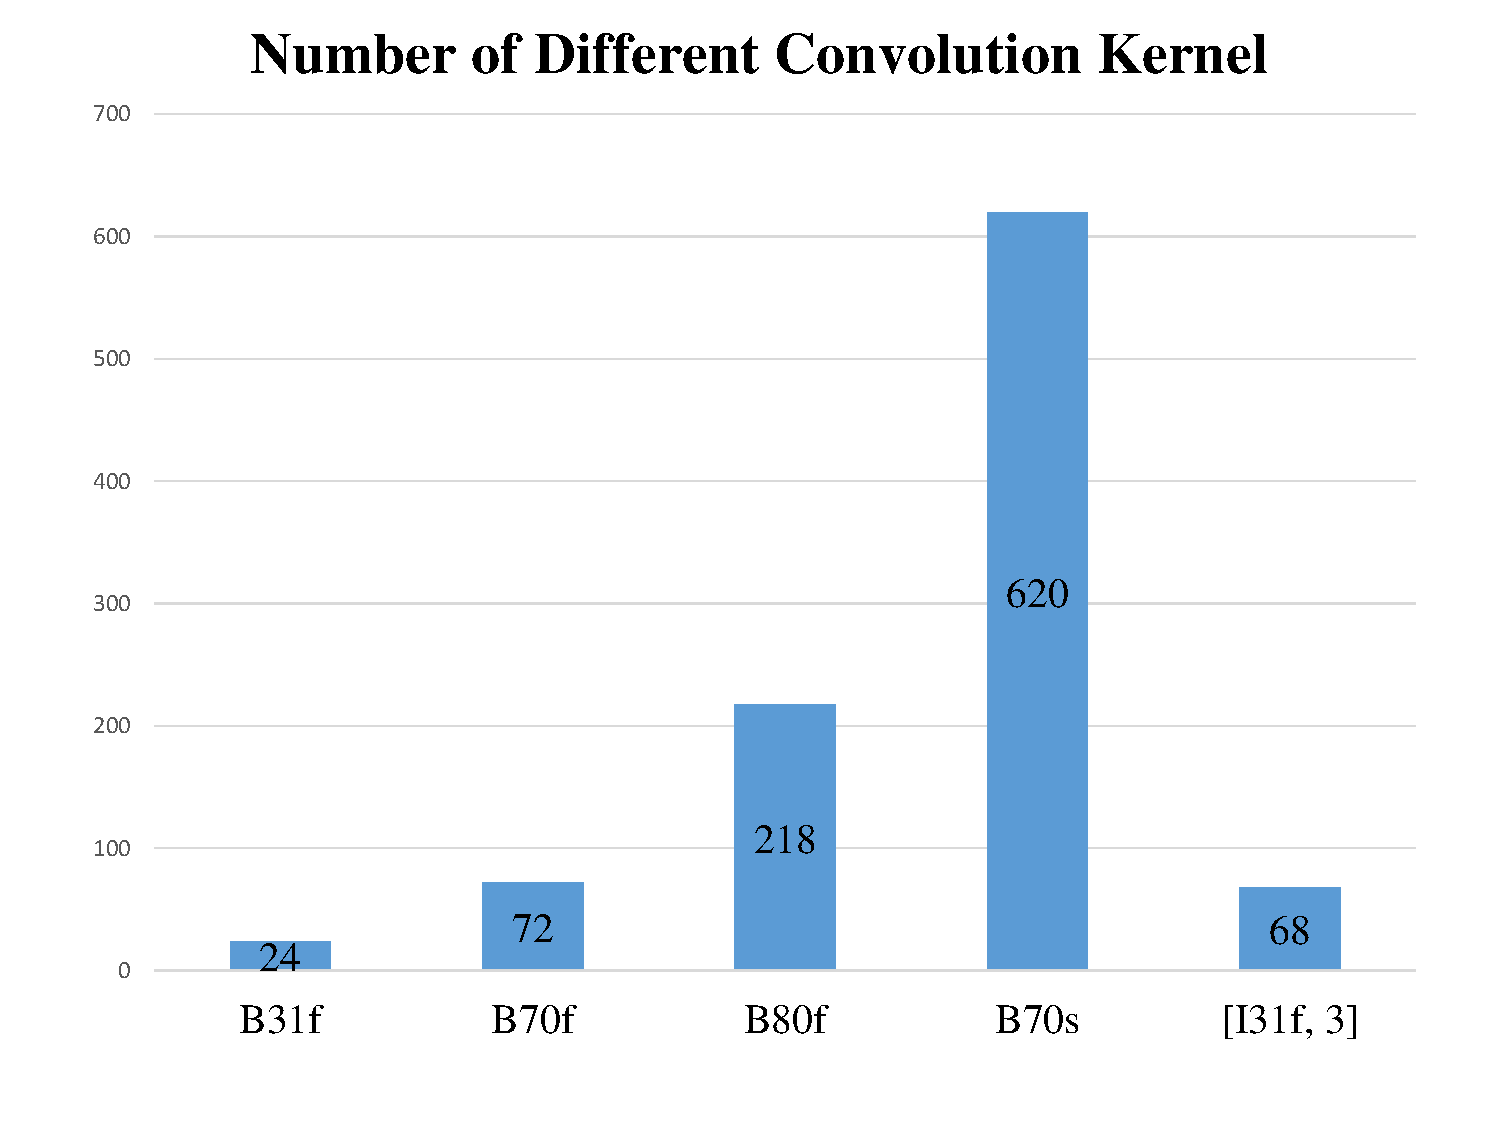
\includegraphics[width=100mm]{NumberofDifferentConvolutionKernel.pdf}}
\vspace{-0cm}
\caption{Number of Different Convolution Kernel}
\vspace{-0cm}
\label{NumberofDifferentConvolutionKernel}
\end{figure}


\begin{table}[htb]
\vspace{-0cm}
\caption{Number of Healthy and Pneumonic Cases in Different Slice-Thickness}
\vspace{-0cm}
\begin{center}
\begin{tabular}{|c|c|c|}
\hline
\textbf{\textit{Slice-Thickness}}& \textbf{\textit{Healthy}}& \textbf{\textit{Pneumonic}}  \\
\hline
1 mm & 0 & 24 \\
1.5 mm  & 1 & 7\\
2 mm & 444 & 386  \\
3 mm & 0 & 127  \\
5 mm & 5 & 8  \\
\hline
Total & 450 & 552 \\
\hline
\end{tabular}
\vspace{-0cm}
\label{distributionofhealthyandpneumonic}
\end{center}
\vspace{-0cm}
\end{table}

\subsubsection{Pre-processing of CT Image Data}
\label{ctimagedata}
There are kinds of image windows for CT reader, such as windows for bone, brain, chest, lungs. Images under different image windows will highlight different tissues of bodies.
In section\ref{ctimagedata}, we can see that each series of CT actually has one specific `Convolution Kernel' and show specific window for CT images directly from raw data. But it may make data inconsistent between different cases. So we transform raw data into HU(Hounsfield Unit) values. The Hounsfield Unit named after Sir Godfrey Hounsfield, is a quantitative scale for describing radio-density, its value is also termed CT number. After transformed into HU value matrices, all slices form CT scans will have the same unit of measure, then we will transform scans according to specific rules.

Following the study in \cite{Shin2017Three} \cite{gao2018holistic}, we transform slices into images using three HU range: lung window [-1000, 400HU], high attenuation [-160, 240HU], low attenuation [-1400, -950HU]. In Fig\ref{3channel} we can see that, compared to original CT image, image in `Lung Window' is brighter, tissues in lungs are clearer and details are enhanced. Image in `High Attenuation' have a clear view of hearts and vessels(in yellow rectangle). `High Attenuation' range also enhance the difference between high dense pathological tissues(in white rectangle) and normal tissues. `Low Attenuation' range highlight abnormal voids in lungs(in red rectangle) which is features of severe lung diseases. 
For each slice, it will generate three 1-channel grey level images(lung window, high attenuation, low attenuation). Then we compress three 1-channel grey level images into one three-channel false color RGB image which fits the requirements of CNN models, as shown in Fig~\ref{3channel}. The `Slice Thickness' between each slice is adjusted into 10mm, and each case will keep 32 slices.

Compared to original CT images, we can clearly see that three-channel images can show more density information about lung tissues. Original CT images are actually grey level images, which can only show lungs with white, black or grey. In this modal, high dense tissues are white, normal lung tissues and low dense tissues are tend to be black. If you want to see details of low dense tissues, you have to adjust the image window to low attenuation range, but meanwhile you will lost the details of high dense tissues. In three-channel images, details of high dense and low dense tissues will both be kept. 
Three-channel fake color images have a larger scale of colors. First of all, high dense tissues will still tend to be white, like bones, high dense tissues in lungs. Second, normal lung tissues will tend to be red, low dense tissues tend to be black, which is very useful when patients have severe lung diseases. 
For example, as shown in Fig~\ref{3channel}, void space(in red rectangle) in original CT images is not very obvious since other normal tissues is in black color too. But in three-channel image, we can clearly notice the difference between normal tissues and low dense tissues. Moreover, the details of high dense tissues(in white rectangle) are still kept. The influence of different HU value ranges will be discussed int section~\ref{effectiveness}.

\begin{figure}[!t]
    \centerline{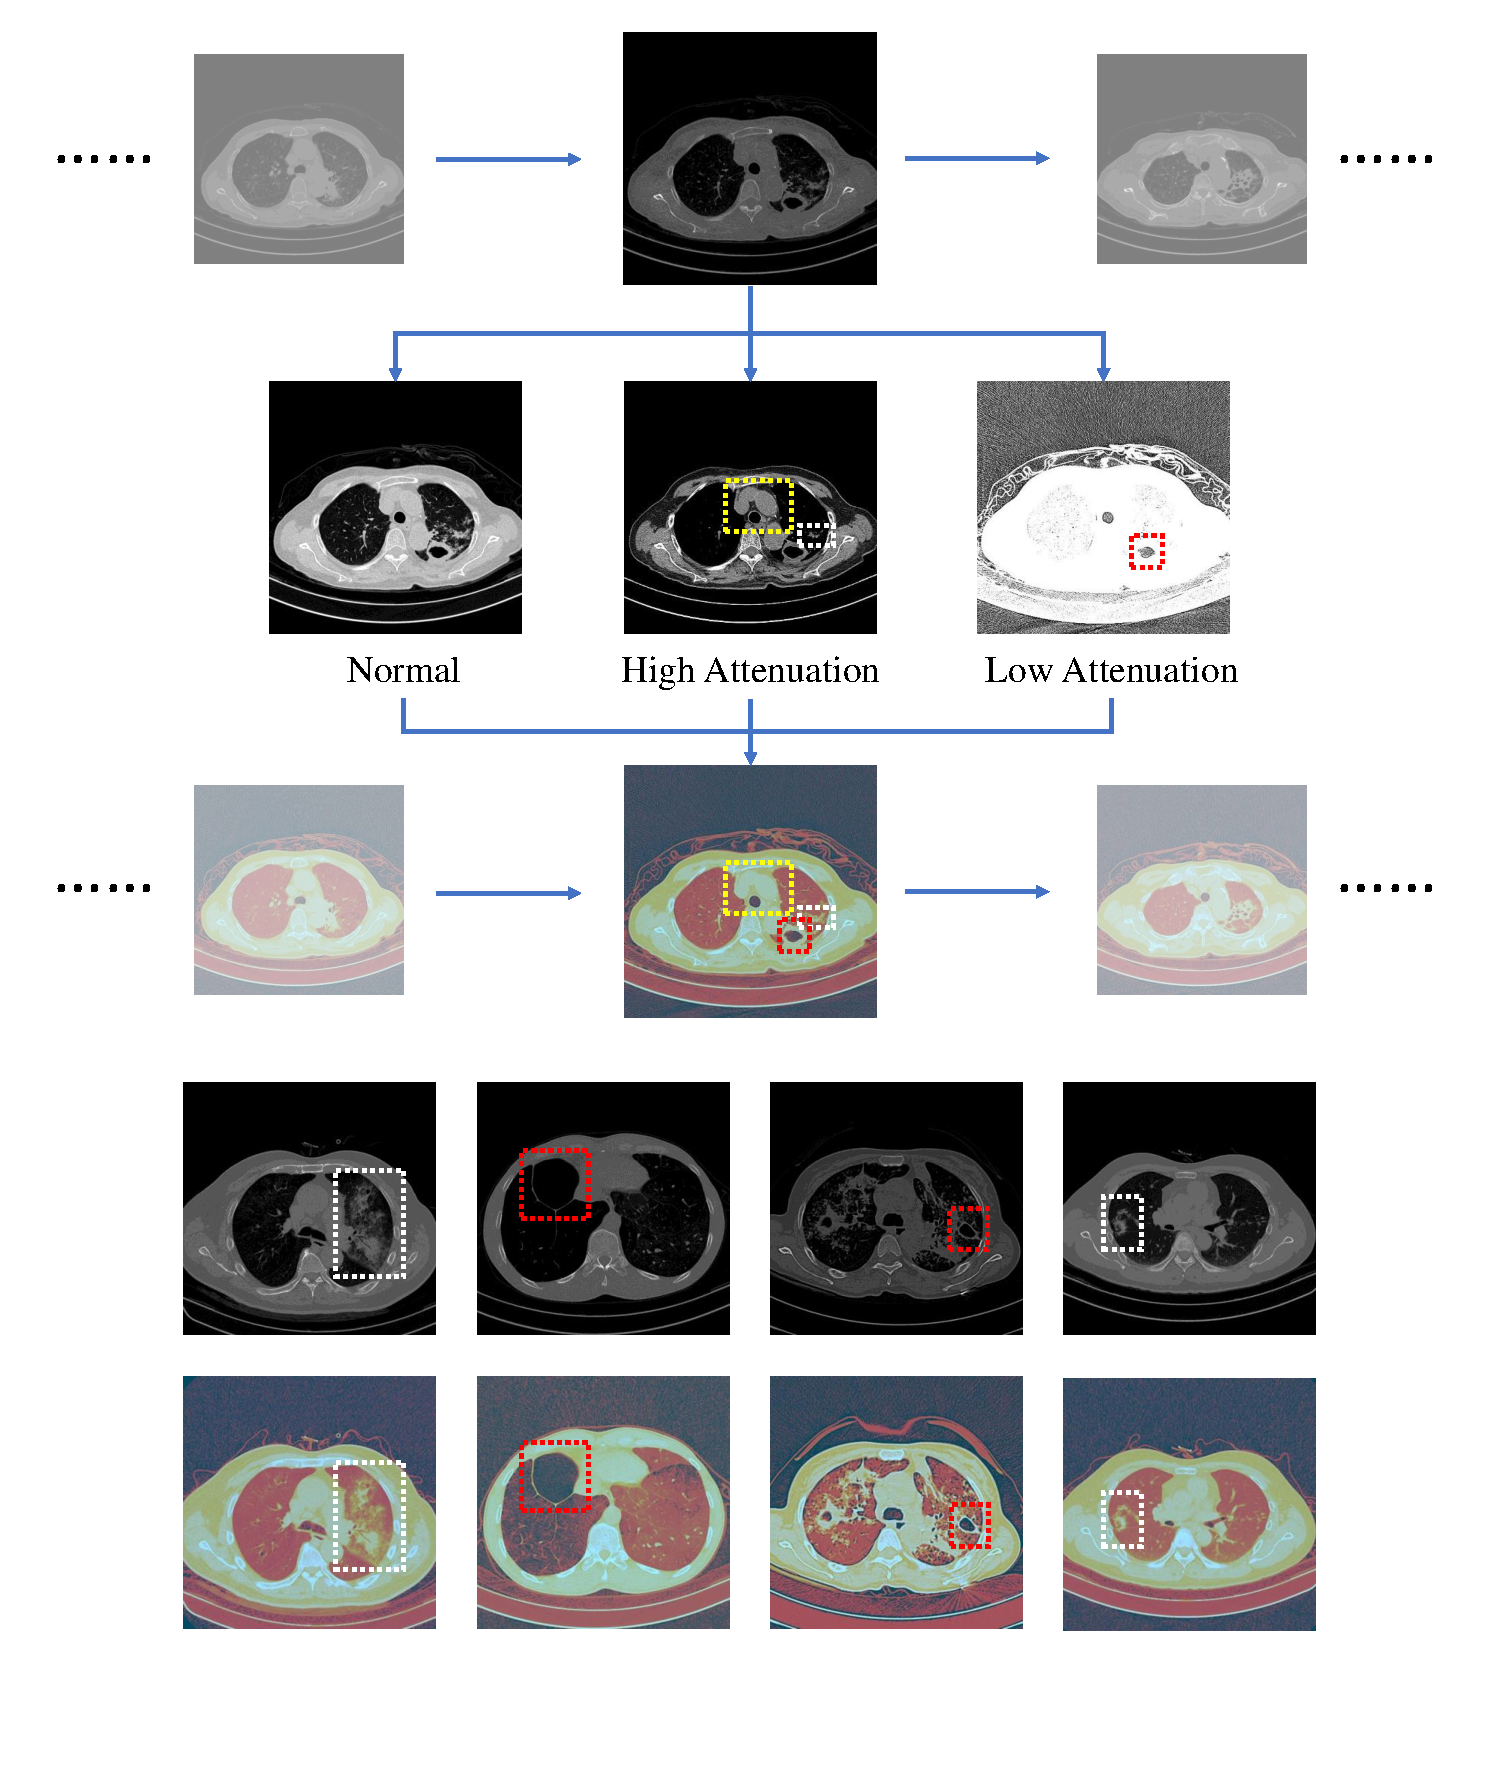
\includegraphics[width=100mm]{3channel.pdf}}
    \vspace{-1cm}
    \caption{Data Pre-precess for CT Scans}
    \vspace{-0cm}
    \label{3channel}
    \end{figure}

\subsubsection{Pre-processing of Patient Age, Gender and Complaints}
\label{textdata}
The pre-process steps of age, gender and complaints is shown in Fig~\ref{textinfo}. For each patient, we have a list of information contains age, gender and complaints. 
For patient age and gender, we transform them into a two-dimensional array. For example, patient in \ref{textinfo} is an adult male, who was born in 1999-10-29. His gender and age will be transformed to $[1, 20]$. A female patient born in 1993 will have $[0, 26]$ to represent her information. $1$ represents male patient, $0$ represents female patient.

For patients' complaints, since we only have Chinese complaints, we have to do Chinese word segmentation. Chinese word segmentation is a very difficult problem so we will take a short cut and use a mature tools: Jieba text segmentation to segment Chinese sentences into Chinese word sequences. Before segmentation, we remove numbers, punctuation marks in order to get a better segmentation results. An example of Chinese word segmentation is shown in green rectangle in Fig~\ref{textinfo}. However, English patient complaints have no need to do segmentation. If you use data from English speaking countries, you may skip this step.
After segmentation, we use word2vec to embed word sequences into vectors. We use CBOW(Continuous Bag-of-Words)\cite{mikolov2013efficient} to capture relationship between words. Since our corpus is very small, we set embedding size as 50, and window size for CBOW as 3. In order to simplify model, we set length of Chinese word sequence to 16 since 16 is the maximum length among all complaint sequences. For those sequences whose length is less than 16, we add `None' to fill up the voids and increase  length to 16. The details of word2vec will not be discussed here. After embedding, each word will be embedded into a vector of 50 dimensions.

Code for data pre-processing has been made into a toolbox and will be released very soon. But we cannot release dataset because of the privacy of patients. We will release model with trained parameters and some sample cases for demo.
\begin{figure}[!t]
    \centerline{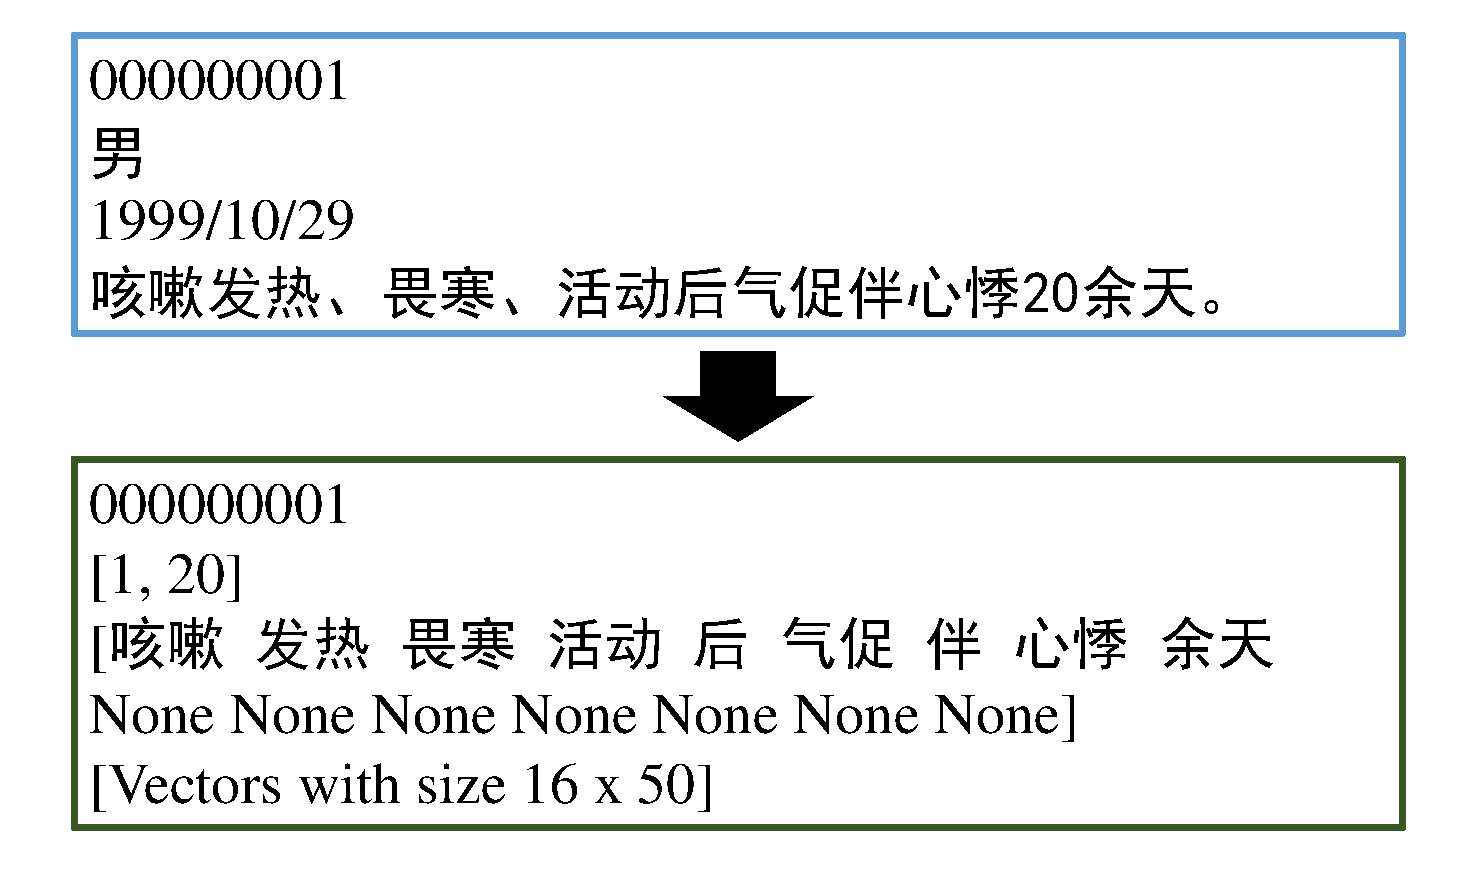
\includegraphics[width=90mm]{textinfo.pdf}}
    \vspace{-0cm}
    \caption{Data Pre-precess for Age, Gender and Complaints}
    \vspace{-0cm}
    \label{textinfo}
    \end{figure}


\subsection{Effectiveness of Three-Channel Image}
\label{effectiveness}
In order to verify the effectiveness of three-channel pre-processing, we output the feature maps of convolutional layer with three-channel images, lung window images, high attenuation images and low attenuation images as show in Fig~\ref{show}. In order to keep experiments environment consistent, all experiments carried on in this part is based on RCNN with ResNet50. In Fig~\ref{show}, images in the first column are original fake color CT images, which are direct outputs from CT slices. The second, the third and the forth columes are feature maps from lung window CNN, high attenuation CNN and low attenuation CNN. Images in the last colume are feature mapes from three-channel CNN.

To verify the effectiveness of difference ranges of HU values, we output middle feature maps of ResNet. More specificity, we output the feature maps after one convolutional layer, one max pooling layer, and three blocks, the size of feature maps are $128 \times 128$, then we resize them into $512 \times 512$. We can see that CNN trained by three-channel images has advantages over CNNs trained by other kinds of images. In the first and the second rows, three-channel CNN can capture the low dense tissues of lungs, which are not very clear in lung window CNN and high attenuation CNN. Low attenuation CNN can notice the low dense tissues, but apparently the details of heart and vessels are ignored in the loa attenuation CNN. 
In the third and the forth row, three-channel CNN still has ability to capture high dense tissues, which is the same as normal CNN and high attenuation CNN, but low attenuation CNN has difficulty in doing this. In the third row, low attenuation CNN cannot distinguish the normal and unnormal tissues. Moreover, in the forth row, low attenuation CNN simply ignores high dense tissues. The last row shows a healthy case. Healthy case has a clear view in lung window CNN, high attenuation CNN and three-channel CNN, but shows nothing in low attenuation CNN.

\begin{figure*}[t]
    \centerline{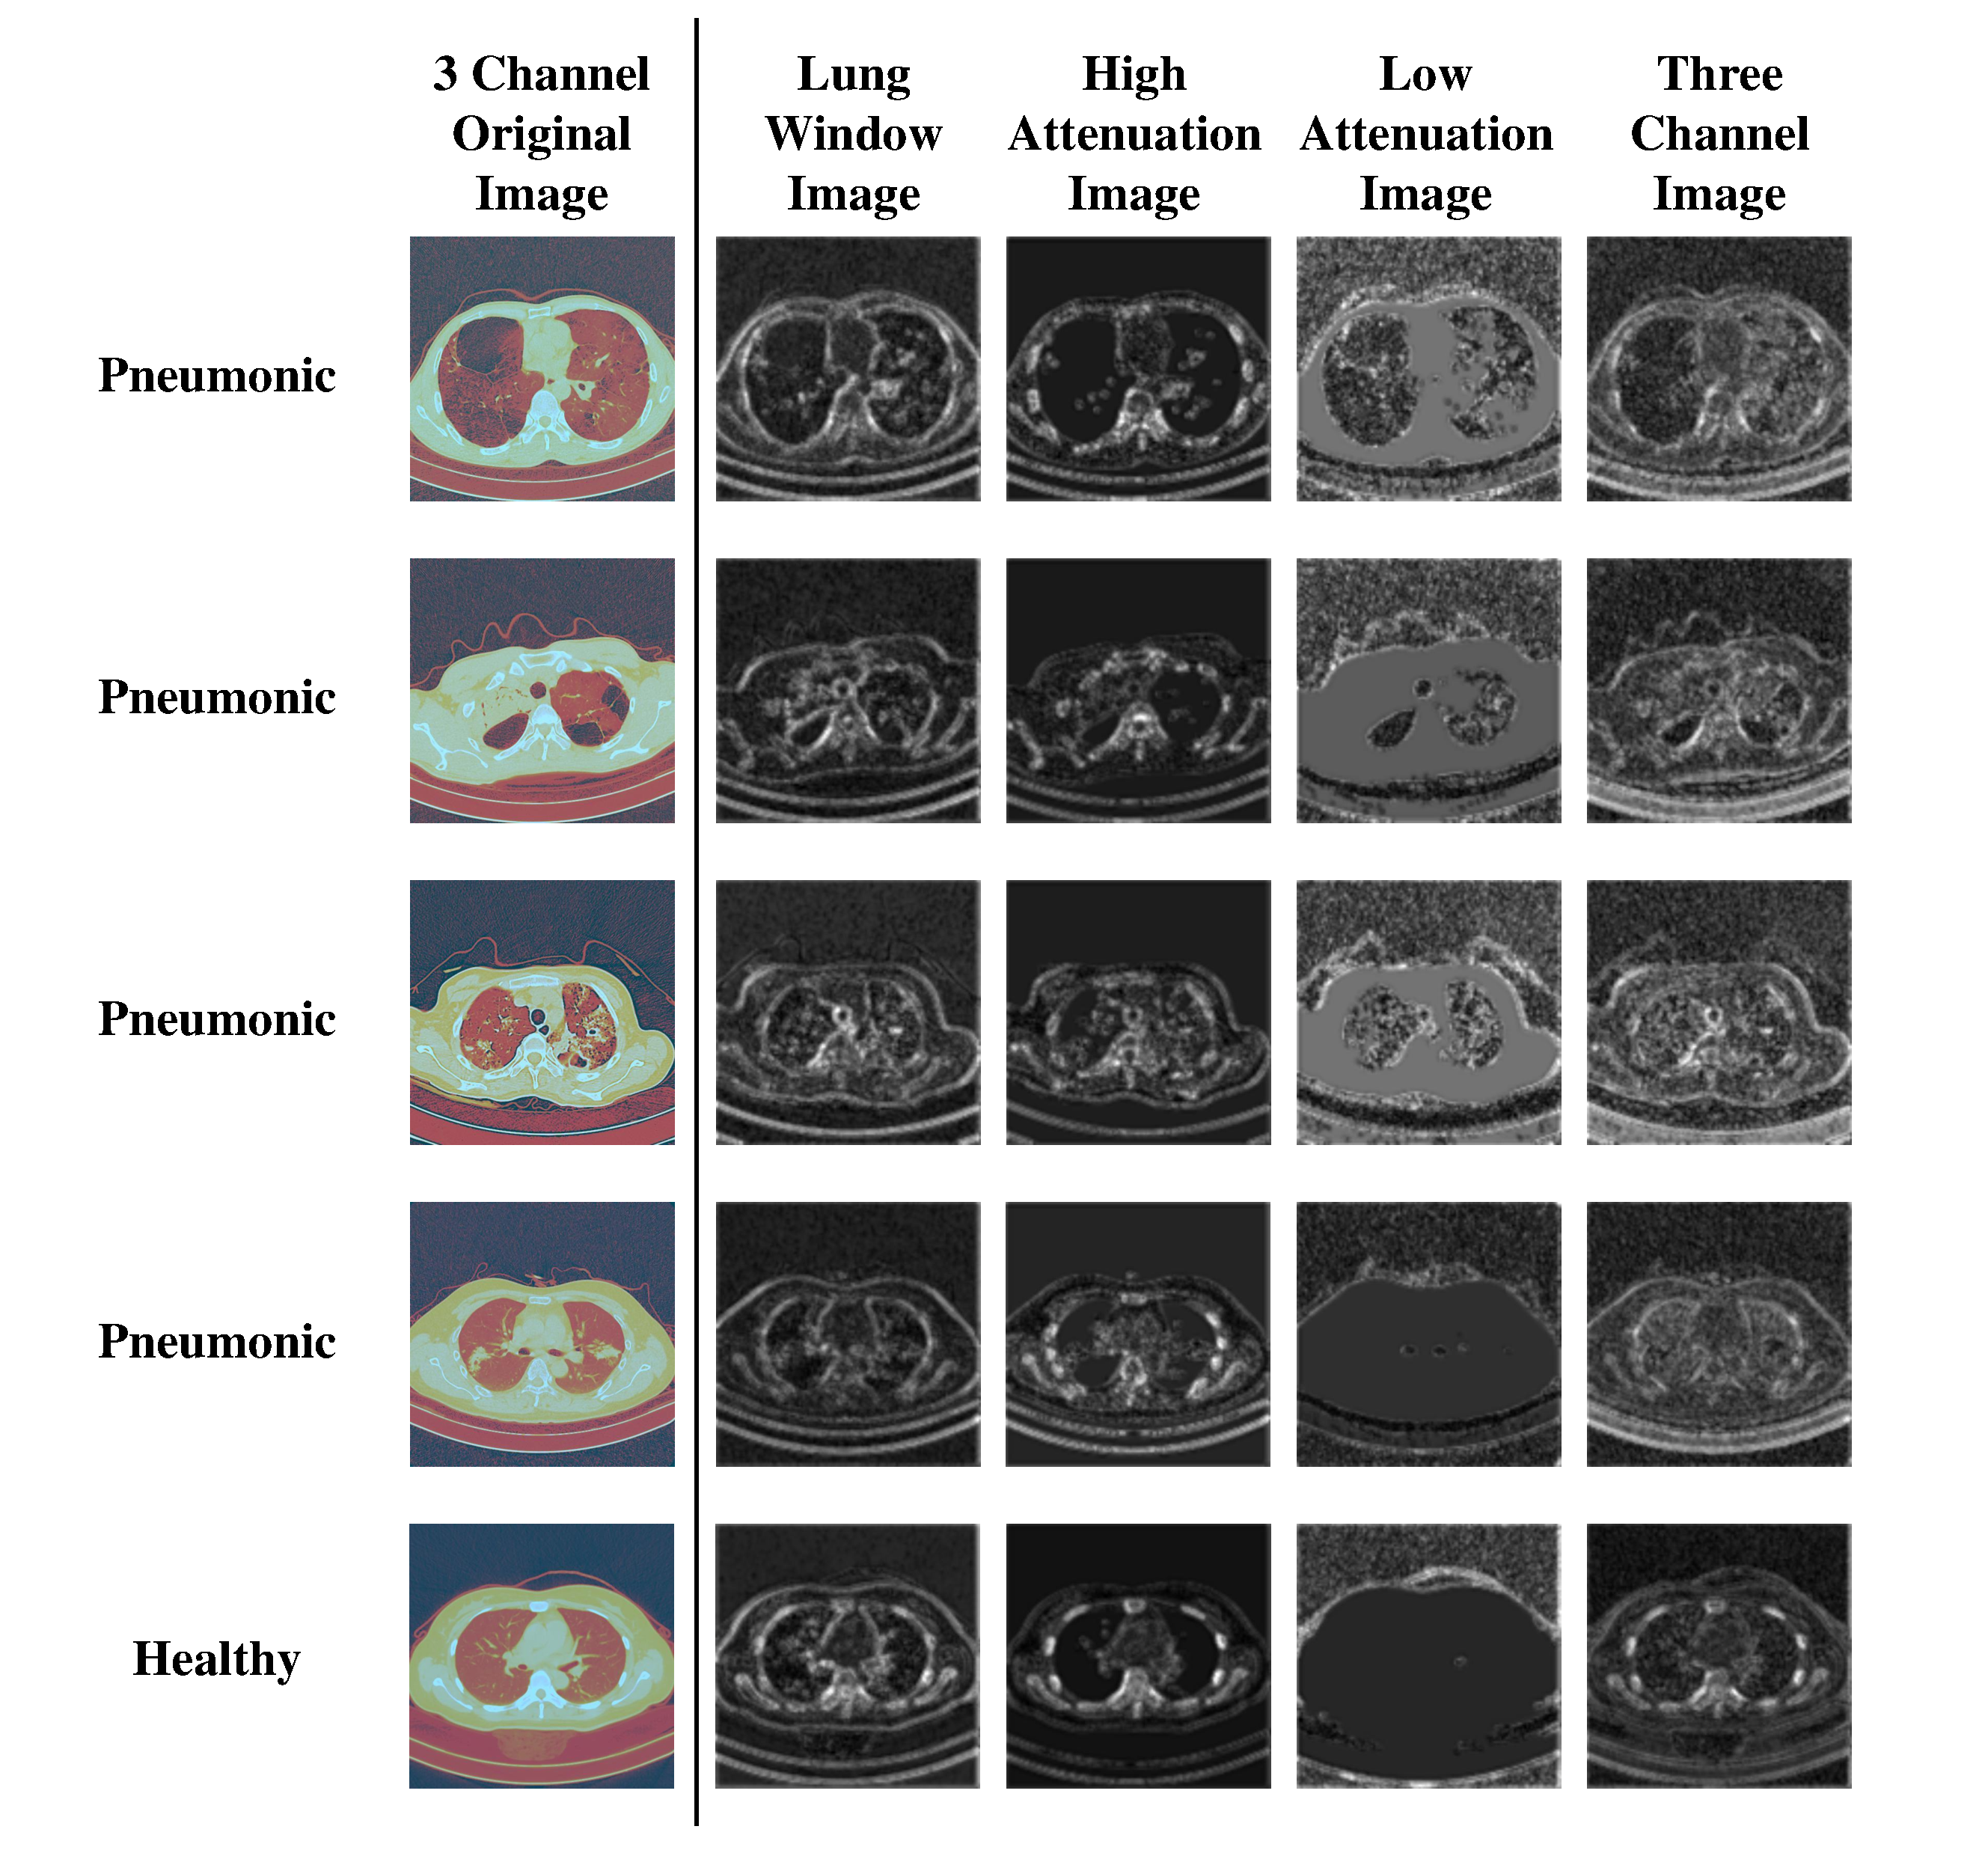
\includegraphics[width=180mm]{show.pdf}}
    \vspace{-0cm}
    \caption{Convolutional Feature Maps from CNN Models Trained by Different Images}
    \vspace{-0cm}
    \label{show}
    \end{figure*}

\subsection{Results}
\label{results}
In order to prove the effect of three-channel images, auxiliary loss and Multimodal Data, we run a lot of experiments to compare with each other, and the results of experiments is shown in Table~\ref{comparison}.

First of all, we do experiments to prove the effect of images with three ranges of HU values and choose the best architecture of RCNN. We can see that RCNN(ResNet), RCNN(GoogLeNet) and RCNN(VGG) trained by three-channel image all have better performance than these models trained by one-channel data. 
For RCNN(VGG), model trained by three-channel image outperforms RCNN(VGG) trained by lung window image in accuracy, specificity and AUROC score. RCNN(VGG) trained by lung window image has better performance in sensitivity, but we can see that it only get 0.626 in specificity, which means this model has not been trained well. 
For RCNN(ResNet) and RCNN(GoogLeNet), we can see that these two models trained by three-channel image perform best compared to those trained by lung window image, high attenuation image and low attenuation image. Especially RCNN(ResNet) trained by three-channel image, it get 0.945 in accuracy, 0.956 in specificity, 0.945 in AUROC score, which are highest in experiments. RCNN(ResNet) trained by lung window image has 0.954 in sensitivity, which is the highest in experiments, but it only achieves 0.824 in specificity and corrupts the performance of whole model. As a result, we use RCNN(ResNet) as our visual feature encoder for CT.

Then we run a experiment to prove the effectiveness of auxiliary loss. We train RCNN(ResNet) with three channel image, but we set $\omega$ to $1$, which means we remove the gradient propagates directly to CNN, this model actually has only one loss. We can see that the performance of RCNN with single loss drops around 1\% in all four indication. It proves that, by using auxiliary loss, CNN will be trained in a better way. 

At last, we run experiments to prove than Multimodal Data can enhance the performance of CAD system. As shown in section~\ref{MMDD}, the output of RCNN($1 \times 256$), features of complaints($1 \times 50$), gender($1 \times 1$) and age($1 \times 1$) will be concatenated together($1 \times 308$) and fused by two fully-connected layers. It is simple, but effective. We can see that MMDD has the highest score in accuracy, specificity and AUROC score. But it achieves 0.936 in sensitivity, 1.8\% lower than the highest 0.954. It means MMDD has the best performance of binary classification according to its AUROC score. We also remove the information about age and gender, we found that MMDD without age and gender has a higher score in sensitivity and lower score in specificity. 
\begin{table*}[htb]
    \vspace{-0cm}
    \caption{Comparison of All Kinds of RCNN and MMDD}
    \vspace{-0cm}
    \begin{center}
    \begin{tabular}{|c|c|c|c|c|c|c|}
    \hline
    \textbf{\textit{Structure}} & \textbf{\textit{Data}}& \textbf{\textit{Accuracy}}  & \textbf{\textit{Sensitivity}} & \textbf{\textit{Specificity}} & \textbf{\textit{AUROC}}& \textbf{\textit{AUROC Rank}}\\
    \hline
    RCNN(VGG) & Lung Window Image & 0.805 & {\bfseries 0.954} &0.626 &0.790 &13\\
    RCNN(GoogLeNet) & Lung Window Image& 0.865 & 0.826 & 0.912 & 0.869 &10\\
    RCNN(ResNet) & Lung Window Image & 0.925 & {\bfseries 0.954} & 0.890 & 0.922 &4\\
    RCNN(GoogLeNet) & High Attenuation Image& 0.880 & 0.853 & 0.912 & 0.883 &8\\
    RCNN(ResNet)& High Attenuation Image& 0.875 & 0.908 & 0.835 & 0.872 &9\\
    RCNN(GoogLeNet) & Low Attenuation Image& 0.860 & 0.890 & 0.824 & 0.857 &12\\
    RCNN(ResNet) & Low Attenuation Image& 0.865 & 0.900 & 0.824 & 0.861 &11\\
    RCNN(VGG) & Three Channel Image& 0.890 & 0.927 &0.846 &0.886 &7\\
    RCNN(GoogLeNet)& Three Channel Image & 0.905 & 0.900 & 0.912 & 0.906 &6\\
    RCNN(ResNet) & Three Channel Image& 0.930 & 0.927 & 0.934 & 0.930 &2\\
    RCNN(ResNet), One Loss & Three Channel Image& 0.920 & 0.917 & 0.923 & 0.920 &5\\
    MMDD & Three Channel Image \& Complaints & 0.925 & 0.945 & 0.901 & 0.923 &3\\
    MMDD & Multimodal Data&  {\bfseries 0.945} & 0.936 & {\bfseries 0.956} & {\bfseries 0.945} &1\\
    \hline
    \end{tabular}
    \vspace{-0cm}
    \label{comparison}
    \end{center}
    \vspace{-0cm}
    \end{table*}

\section{Discussion}
\label{discuss}
The validation loss and accuracy during training is shown in Fig~\ref{aac} and Fig~\ref{loss}. We can see that in Fig~\ref{aac}, MMDD can achieve higher accuracy at the first phase of training, but RCNN(ResNet), RCNN(GoogLeNet) and RCNN(ResNet) with single loss perform better after. MMDD's performance outperforms other methods again after 27000 training step. We can also see that RCNN(ResNet), RCNN(ResNet) with single loss have similar performance during training, but RCNN(ResNet) with auxiliary loss perform a little bit better than RCNN(ResNet) with single loss at the end of training. For RCNN(GoogLeNet), it converge slower than RCNN(ResNet) and RCNN(ResNet) with single loss, and has a lower accuracy in the end. Without age and gender, MMDD has similar performance compared to RCNN(ResNet) with single loss. According to the experiments above, we can see that information about age and gender can improve accuracy to 0.7 at the very beginning, it means the dataset we are using must be influenced by some certain distribution. So we count the number of male patients and female patients in healthy cases and pneumonic cases(Table~\ref{malefemale}) and number of patients in different ages(Table~\ref{differentages}). 

\begin{figure}[t]
    \centerline{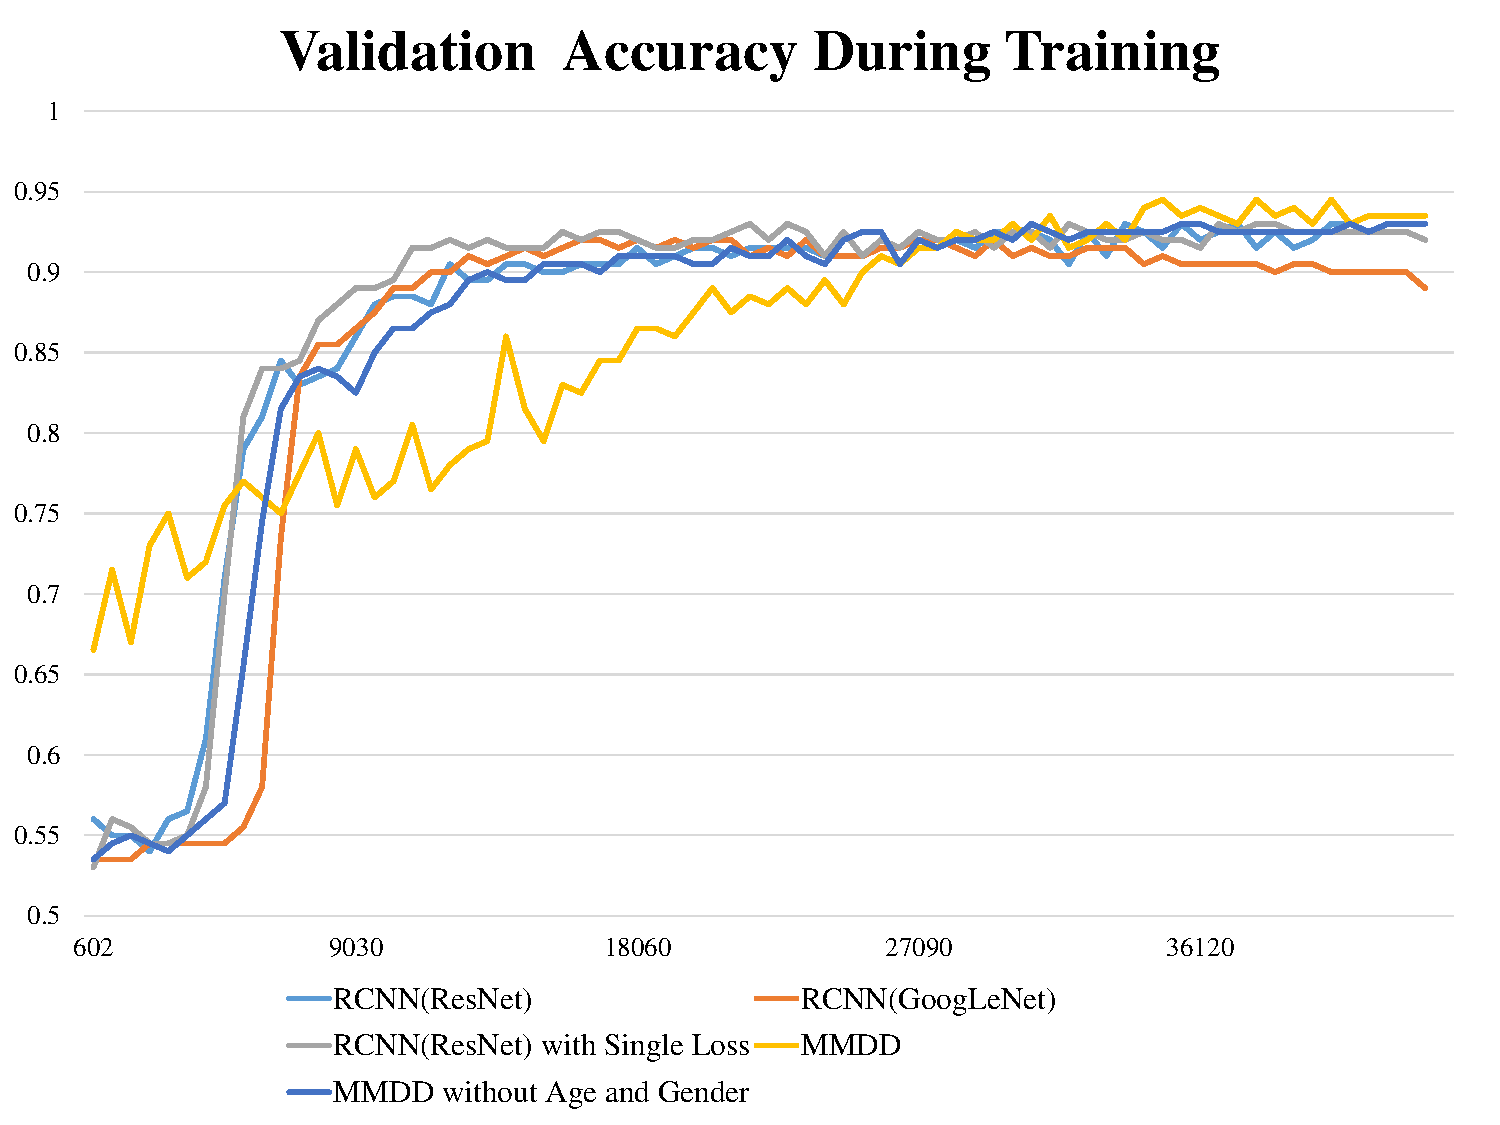
\includegraphics[width=90mm]{aac.pdf}}
    \vspace{-0cm}
    \caption{Validation Accuracy During Training}
    \vspace{-0cm}
    \label{aac}
    \end{figure}

\begin{figure}[t]
    \centerline{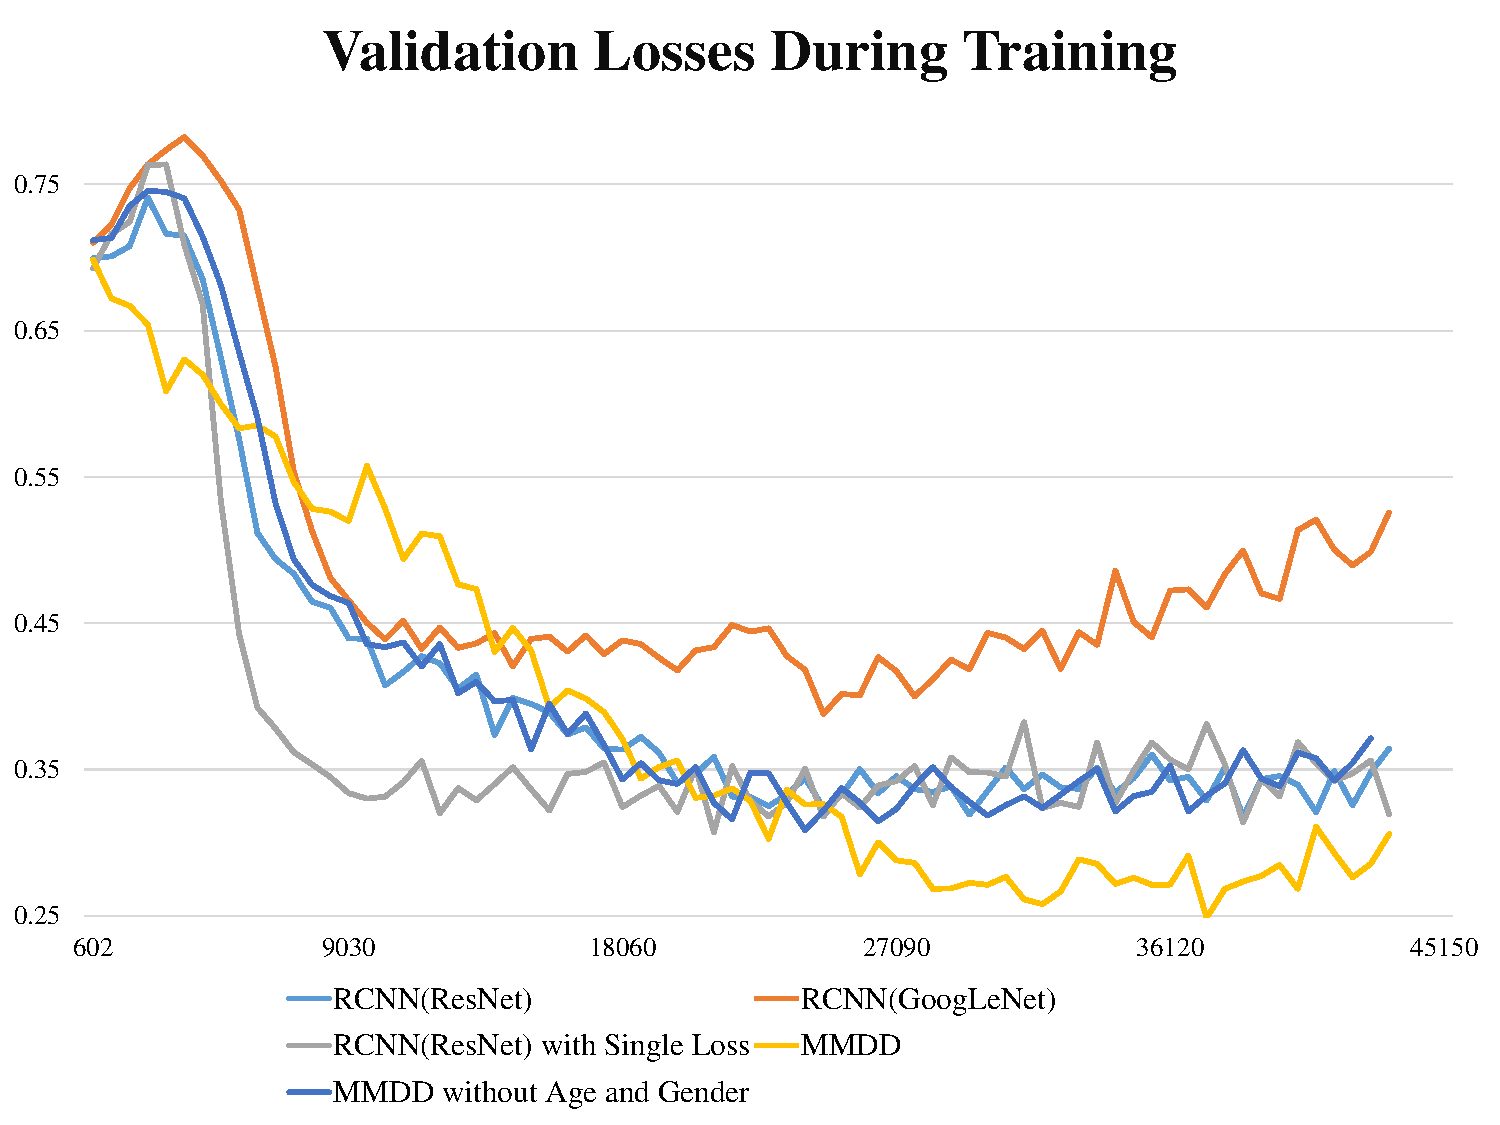
\includegraphics[width=90mm]{losses.pdf}}
    \vspace{-0cm}
    \caption{Validation Loss During Training}
    \vspace{-0cm}
    \label{loss}
    \end{figure}


In Table~\ref{malefemale}, we can see that a male patient has a larger chance of being pneumonic. In 601 male cases, about 60\% of them are pneumonic, however, in 401 female cases, only 47.6\% are pneumonic. This may be related to smoking since male in Chinese suffer a serious smoking problem. 
In Table~\ref{differentages}, we can see that age is also related to the chance of being pneumonic. People turn to hospital or clinic may have noticed that something goes wrong about their healthy condition, but we can still see that people older than 40 have much larger chance of being pneumonic. There are about half of healthy cases between 40-50, but this number drops so quickly that it goes down to 28.8\% between 50-60. It is not hard to understand this phenomenon, since young people are very sensitive about their healthy condition, they will go to have physical examination as long as they feel uncomfortable, even if they have a lower chance of having pneumonia. However, old people have to face up with another condition. Most old people only go to hospital or clinic when their conditions are very bad. It reminds us that there is a lot of work need to be done about old people health care.


\begin{table}[htb]
    \vspace{-0cm}
    \caption{Number of Male and Female Patients in Healthy and Pneumonic Cases}
    \vspace{-0cm}
    \begin{center}
    \begin{tabular}{|c|c|c|c|c|}
    \hline
    \textbf{\textit{}} & \textbf{\textit{Healthy}} & \textbf{\textit{Pneumonic}}& \textbf{\textit{Total}}& \textbf{\textit{Percentage*}} \\
    \hline
    Male & 240 & 361 & 601 & 60.1\%\\
    Female & 210 & 191 & 401 &47.6\% \\
    \hline
    \textbf{\textit{Total}} & 450 & 552 & 1002 & 55.1\% \\
    
    \hline
    \end{tabular}
    \vspace{0.1cm}
    \label{malefemale} \\
    \footnotesize{Percentage* is Percentage of Pneumonia Patients}

    \end{center}

    \vspace{-0.0cm}
    \end{table}

\begin{table}[htb]
    \vspace{-0cm}
    \caption{Number of Healthy and Pneumonic Cases in Different Ages}
    \vspace{-0cm}
    \begin{center}
    \begin{tabular}{|c|c|c|c|c|}
        \hline
        \textbf{\textit{}} & \textbf{\textit{Healthy}} & \textbf{\textit{Pneumonic}}& \textbf{\textit{Total}}& \textbf{\textit{Percentage*}} \\
    \hline
    0-10 & 6 & 1 & 7 & 14.3\%\\
    10-20 & 31 & 2 & 33 & 6.1\%\\
    20-30 & 122 & 30 & 152 & 19.7\%\\
    30-40 & 124 & 45 & 169 &26.6\%\\
    40-50 & 109 & 108 & 217 &49.8\%\\
    50-60 & 53 & 131 & 184 &71.2\%\\
    60-70 & 5 & 126 & 131 &96.2\%\\
    70-80 & 0 & 82 & 82 &100\%\\
    $>90$& 0 & 27 & 27 &100\%\\
    \hline 
    \textbf{\textit{Total}} & 450 & 552 & 1002 & 55.1\% \\
    
    \hline
    \end{tabular}
    \vspace{0.1cm}
    \label{differentages}\\
    \footnotesize{Percentage* is Percentage of Pneumonia Patients}

    \end{center}
    \vspace{-0.0cm}
    \end{table}


In Fig~\ref{loss}, we can see that RCNN(GoogLeNet) has the highest loss at the end of training, so it perform the worst in accuracy. RCNN(ResNet) and MMDD without age and gender has similar performance. RCNN(ResNet) with single loss drops quickly at first, but its loss is very close to RCNN(ResNet) in the end. MMDD has the lowest loss at beginning of training, even if it has the highest loss for a moment during training, it has the lowest loss after 27090 training steps. This phenomenon is not hard to understand. Since our dataset is influenced by distribution, MMDD has the lowest loss at beginning, which is corresponding to the phenomenon in Fig~\ref{aac}. But MMDD has more parameters to train, so its loss drops slower than others.






% An example of a floating figure using the graphicx package.
% Note that \label must occur AFTER (or within) \caption.
% For figures, \caption should occur after the \includegraphics.
% Note that IEEEtran v1.7 and later has special internal code that
% is designed to preserve the operation of \label within \caption
% even when the captionsoff option is in effect. However, because
% of issues like this, it may be the safest practice to put all your
% \label just after \caption rather than within \caption{}.
%
% Reminder: the "draftcls" or "draftclsnofoot", not "draft", class
% option should be used if it is desired that the figures are to be
% displayed while in draft mode.
%
%\begin{figure}[!t]
%\centering
%\includegraphics[width=2.5in]{myfigure}
% where an .eps filename suffix will be assumed under latex, 
% and a .pdf suffix will be assumed for pdflatex; or what has been declared
% via \DeclareGraphicsExtensions.
%\caption{Simulation results for the network.}
%\label{fig_sim}
%\end{figure}

% Note that the IEEE typically puts floats only at the top, even when this
% results in a large percentage of a column being occupied by floats.


% An example of a double column floating figure using two subfigures.
% (The subfig.sty package must be loaded for this to work.)
% The subfigure \label commands are set within each subfloat command,
% and the \label for the overall figure must come after \caption.
% \hfil is used as a separator to get equal spacing.
% Watch out that the combined width of all the subfigures on a 
% line do not exceed the text width or a line break will occur.
%
%\begin{figure*}[!t]
%\centering
%\subfloat[Case I]{\includegraphics[width=2.5in]{box}%
%\label{fig_first_case}}
%\hfil
%\subfloat[Case II]{\includegraphics[width=2.5in]{box}%
%\label{fig_second_case}}
%\caption{Simulation results for the network.}
%\label{fig_sim}
%\end{figure*}
%
% Note that often IEEE papers with subfigures do not employ subfigure
% captions (using the optional argument to \subfloat[]), but instead will
% reference/describe all of them (a), (b), etc., within the main caption.
% Be aware that for subfig.sty to generate the (a), (b), etc., subfigure
% labels, the optional argument to \subfloat must be present. If a
% subcaption is not desired, just leave its contents blank,
% e.g., \subfloat[].


% An example of a floating table. Note that, for IEEE style tables, the
% \caption command should come BEFORE the table and, given that table
% captions serve much like titles, are usually capitalized except for words
% such as a, an, and, as, at, but, by, for, in, nor, of, on, or, the, to
% and up, which are usually not capitalized unless they are the first or
% last word of the caption. Table text will default to \footnotesize as
% the IEEE normally uses this smaller font for tables.
% The \label must come after \caption as always.
%
%\begin{table}[!t]
%% increase table row spacing, adjust to taste
%\renewcommand{\arraystretch}{1.3}
% if using array.sty, it might be a good idea to tweak the value of
% \extrarowheight as needed to properly center the text within the cells
%\caption{An Example of a Table}
%\label{table_example}
%\centering
%% Some packages, such as MDW tools, offer better commands for making tables
%% than the plain LaTeX2e tabular which is used here.
%\begin{tabular}{|c||c|}
%\hline
%One & Two\\
%\hline
%Three & Four\\
%\hline
%\end{tabular}
%\end{table}


% Note that the IEEE does not put floats in the very first column
% - or typically anywhere on the first page for that matter. Also,
% in-text middle ("here") positioning is typically not used, but it
% is allowed and encouraged for Computer Society conferences (but
% not Computer Society journals). Most IEEE journals/conferences use
% top floats exclusively. 
% Note that, LaTeX2e, unlike IEEE journals/conferences, places
% footnotes above bottom floats. This can be corrected via the
% \fnbelowfloat command of the stfloats package.




\section{Conclusion}
\label{conclude}
In this study, we propose a novel model, MMDD(Multimodal Data Diagnosis), which combines CT visual features with patients' age, gender and complaints. In MMDD, CT scans will be treated like videos, and analyzed by RCNN(Recurrent Convolutional Neural Network), complaints will be transformed into word vectors by word2vec and analyzed by LSTM. Features from CT images and complaints will be fused together with patients' age and gender. All these features will be used to classify cases into healthy cases or pneumonic cases.

We analyze 1002 cases(450 healthy cases and 552 pneumonic cases). In fact, 1002 cases is far small than `big data', so our model's performance is restricted by data distribution and quality. However, in clinical practice, it is very difficult to construct a big scale medical dataset for deep learning, cause raw data is affected by radiologists' personal habits, data acquisition equipments, and hospital work rules. Our future work will focus on methods of data pre-processing which can over come difficulties mentioned above.
Moreover, our future work will also focus on fusing more source of information, like medical history, family history, blood test and other information which will be considered during clinical practice. All works above will be carried out under the premise of respecting the privacy of the patients.
 




% if have a single appendix:
%\appendix[Proof of the Zonklar Equations]
% or
%\appendix  % for no appendix heading
% do not use \section anymore after \appendix, only \section*
% is possibly needed

% use appendices with more than one appendix
% then use \section to start each appendix
% you must declare a \section before using any
% \subsection or using \label (\appendices by itself
% starts a section numbered zero.)
%


% \appendices
% \section{Proof of the First Zonklar Equation}
% Appendix one text goes here.

% % you can choose not to have a title for an appendix
% % if you want by leaving the argument blank
% \section{}
% Appendix two text goes here.


% use section* for acknowledgment
\section*{Acknowledgment}


The authors would like to thank...


% Can use something like this to put references on a page
% by themselves when using endfloat and the captionsoff option.
\ifCLASSOPTIONcaptionsoff
  \newpage
\fi



% trigger a \newpage just before the given reference
% number - used to balance the columns on the last page
% adjust value as needed - may need to be readjusted if
% the document is modified later
%\IEEEtriggeratref{8}
% The "triggered" command can be changed if desired:
%\IEEEtriggercmd{\enlargethispage{-5in}}

% references section

% can use a bibliography generated by BibTeX as a .bbl file
% BibTeX documentation can be easily obtained at:
% http://mirror.ctan.org/biblio/bibtex/contrib/doc/
% The IEEEtran BibTeX style support page is at:
% http://www.michaelshell.org/tex/thebibliography/bibtex/
\bibliographystyle{IEEEtran}
% argument is your BibTeX string definitions and bibliography database(s)
\bibliography{refs}
%
% <OR> manually copy in the resultant .bbl file
% set second argument of \begin to the number of references
% (used to reserve space for the reference number labels box)





% biography section
% 
% If you have an EPS/PDF photo (graphicx package needed) extra braces are
% needed around the contents of the optional argument to biography to prevent
% the LaTeX parser from getting confused when it sees the complicated
% \includegraphics command within an optional argument. (You could create
% your own custom macro containing the \includegraphics command to make things
% simpler here.)
%\begin{IEEEbiography}[{\includegraphics[width=1in,height=1.25in,clip,keepaspectratio]{mshell}}]{Michael Shell}
% or if you just want to reserve a space for a photo:

\begin{IEEEbiography}{Michael Shell}
Biography text here.
\end{IEEEbiography}

% if you will not have a photo at all:
\begin{IEEEbiographynophoto}{John Doe}
Biography text here.
\end{IEEEbiographynophoto}

% insert where needed to balance the two columns on the last page with
% biographies
%\newpage

\begin{IEEEbiographynophoto}{Jane Doe}
Biography text here.
\end{IEEEbiographynophoto}

% You can push biographies down or up by placing
% a \vfill before or after them. The appropriate
% use of \vfill depends on what kind of text is
% on the last page and whether or not the columns
% are being equalized.

%\vfill

% Can be used to pull up biographies so that the bottom of the last one
% is flush with the other column.
%\enlargethispage{-5in}



% that's all folks
\end{document}


